
\begin{savequote}[8cm]

  \qauthor{}
\end{savequote}



\chapter{Performance, team click, social bonding among Beijing rugby players\label{chap:ethnoResults}}

\minitoc






                                      \begin{CJK}{UTF8}{gbsn}

\section{Ethnographic evidence for a relationship between joint action and social bonding}


In this results section, I outline ethnographic evidence according to the theoretical predictions set out in this dissertation concerning joint action and social bonding. Results are divided into three sections: 1) perceptions of performance in joint action, 2) team click, and 3) group membership.


%\section{Introduction}

%Restate the question: come together and move together

%Restate context
%Specific terrain (Chap5)
%predictions


\section{Perceptions of performance in joint action}
Unsurprisingly, ethnographic observations revealed that perceptions of team and individual performance of the on-field requirements of rugby were a central dimension to athletes' experience of the rugby program at the Institute.  As explained in previous chapters, most of the athletes in the rugby program at the Institute had recently transitioned to rugby from other sports, or otherwise had no specific background in sport before coming to the Institute.  Rugby's minnow status in China means that its technical requirements are not widely known or understood beyond the small community of athletes who play the sport.  Thus, from a very low base of prior knowledge, athletes who take up the sport for the first time are forced to develop fluency in the technical and social competencies associated with rugby.  The ability to effectively coordinate behaviour with others, both on and off the field, is therefore crucial to an athlete's ability to navigate the rugby program at the Institute and access the incentives available.  If an athlete wishes to pursue a future through rugby, doing so hinges predominantly on effectively an individual can contribute to the success of on-field joint action.

%In addition, the concept of living and training full time with a group of non-kin is, as a general rule, a relatively novel social requirement for most athletes.  Millions of Chinese university aged students leave home and cohabitate in university dormitories, prior to which point most live at home with their immediate families.

%Starting at time with almost zero prior experience of rugby, athletes must learn the technical skills of passing, tackling, running, kicking---and all of these these individual technical components must be harmonised in joint action with other athletes on the same team, as well as against opposition athletes.  Off the field, as discussed in the previous chapter, the rugby program at the Institute requires athletes to navigate a complex social environment, structured by hierarchical relations of power.

\subsection{The challenge of joint action in rugby}

It soon became obvious that rugby's joint action requirements posed a significant challenge for athletes attempting to learn the game from scratch.  During semi-interviews, within the general theme questioning regarding of the costs and benefits of adherence to rugby, I asked athletes what they thought was ``the most difficult part of rugby'' (你觉得橄榄球最难的一部分是什么).  I deliberately left the question open to interpretation, and if asked to clarify, I followed up by using the compound \textit{kunan} (困难), to emphasise the challenging dimension of difficulty, i.e. ``what is the most \textit{challenging} part of rugby?'' (橄榄球最\textbf{困难}的一部分是什么?).

Of the 20 athletes who responded directly to this question (in the remaining six interviews either I did not ask this question, or athletes did not respond to the question), all 20 interpreted it as a question about rugby's on-field demands.  11 athletes cited an aspect of rugby that related to on-field coordination of behaviour in joint action, such as decision making in attack, ``awareness'' (\textit{yishi} 意识) or vision (\textit{shiye} 视野)in game play, coordinating running lines, executing planned plays, and so on.  Seven athletes cited aspects of individual performance, such as tackling, speed in defence, footwork in attack. The remaining two athletes cited both an aspect that was related to coordination of behaviours with others, as well as an aspect of individual performance.

In his interview, senior athlete and Beijing local Su Hailiang summed up the feeling of being a new athlete without any foundation in rugby:

\begin{quote}
    I think the hardest thing---well it was all really hard.  At the time when I couldn't do anything, when my body development wasn't that good, I wasn't that strong.  Basic skills, ball skills, planned moves, etc. [were all not very good].
\end{quote}

\begin{quote}
    我觉得最困难的,都挺困难的,当时什么都不会,身体素质也没那么好,没有那么强壮,也没有那么好,身体素质。基本功、球技、记战术什么的。
\end{quote}

This passage suggests that an athlete's initial induction into the rugby program could be overwhelming due to rugby's many diverse requirements.  As unruly undergrad Fang Chao explains:

\begin{quote}
  The hardest thing about rugby is all of the small details. Rugby is such a comprehensive sport, and playing in a real game is very different from training. I remember when was playing a tournament in 2014, at the time I had only just started training (for rugby).  As soon as I took the field my whole brain was blank.  Now I am a bit better, my vision is broader.
\end{quote}

\begin{quote}
  橄榄球最难的一部分是很多小细节吧。橄榄球是很全面的项目,打比赛跟训练还是有区别的。 14年的时候打比赛,那时候刚练,一上场整个脑子就空白了,现在会好一点,视野也开阔了。
\end{quote}

In his response, Fangchao draws attention to the difficulty associated with the ``on-line'' and ``in-the-moment'' demands of joint action in rugby.  When he first started playing in real rugby matches, the pressure of being on the field and in the moment meant that there was no time for him to think or see.

Results suggested that team performance posed a more significant challenge than individual performance.  As discussed in Chapter~\ref{chap:researchSetting} Section ~\ref{sect:jointActionRugby}, almost all action in rugby can be classed as joint action.  From the point of view of the action of a single team, however, joint action in rugby can be grouped into two modes: aspects of \textit{team performance} and aspects of \textit{individual performance}.  Team performance usually entails joint action that requires explicit coordination with teammates (such as coordination of attack and defensive line, passing between two or more players, etc).  Components of individual performance, by contrast, entails a focus on individual actions that contribute to larger joint action goals (such as tackling, individual passing, effectiveness in contact encounters at the breakdown, etc.)

As Wang Zhenfeng, a tall and extremely talented (but still relatively inexperienced) senior athlete, explained:

\begin{quote}
  For me, it's probably the decision making with ball in hand: after you get the ball, how do you create opportunities for others---I think that's especially difficult.  For me, I think breaking the line or attack or whatever...breaking the line or stepping and so on...I'm ok at all of these things [individual components of performance], but if you ask me to create an opportunity for someone else after I have broken the line---that's when I find it difficult.
\end{quote}

\begin{quote}
  对我来讲应该是球的分化,拿到球之后分化给别人创造机会我觉得特别难。我觉得突破或进攻还是干嘛的,去突变向什么的对我来说都还好,但是让我即能突然后给别人创造机会我觉得很难。
\end{quote}

In this sense, it is not only the on-line dimension of rugby that Wang finds challenging, but also the fact that he must create opportunities for others.  Wang Zhankun, a young and promising kid student from Chaoyang school expressed a similar sentiment:

\begin{quote}
  I’d say the ability to adjust to being on the field in a game.  When I’m on the field I can only see those few people who are close to me, when I’m tired I feel like I can’t see anything, like there could be a gap, or an opportunity, but often I can see it.
\end{quote}

\begin{quote}
  场上的适应能力吧。我在场上只能看到离自己近的几个人,累的时候感觉看不到所有,可能空档啊、机会啊经常看不到.
\end{quote}

The theme of ``awareness'' (\textit{yishi} 意识) was prominent in answers to this question. Of the 13 athletes who cited coordination of behaviour with others as the (or one of the) most difficult aspects of rugby,  six athletes mentioned awareness directly.  Of these six, five mentioned awareness (\textit{yishi}) and one specified ``continuous on-field awareness'' (在场上连续意识).  Of the remaining seven athletes, three talked about on-field coordination with others (\textit{peihe} 配合), two talked about on field decision-making (\textit{panduan nengli} 判断能力), and two talked about planned running lines (\textit{paowei} 跑位) and team moves (\textit{zhanshu} 战术).

Bao Yuhan, an unruly undergrad and Beijing local, expressed to his experience of the challenge of awareness on the field:

  \begin{quote}
    (I think its about) maintaining continuous on-field awareness.  Often I'm never thinking that many steps ahead.  Sometimes when I break the line, once I break through I can't keep on going.  Suppose like that one time in Shanghai in 2014, I gave the ball to Wang Zhenfeng and he broke through, and then no one followed him.  I stood there looking at him run from where I passed the ball, I was so tired I couldn't do anything... As soon as I realised what was happening, I was like ``Oh! Quick get after him!'' In the end we were one step away---only one step away from losing the ball.
  \end{quote}

  \begin{quote}
    在场上连续意识. 我总是想的不是那么多翻。有时候突破的时候,突破了不会再打。假如在上海14年我给王贞丰突破了,然后没人追上了,我在原地累得不行了看着,我一看,''哦!快追上!''最后差一步,就差一点会丢球。
  \end{quote}

These passages taken from semi-structured interviews suggest that rugby's on-field demands in joint action place severe constraints on athletes' ability to be (consciously) aware of the environment around them, including the actions and intensions of others.  Like Wang Zhankun above, Bao Yuhan also suggests that physiological fatigue has an impact on ability to maintain awareness.  Thus, in addition to the time pressure and cognitive complexity of joint action in rugby, the role of exertion and fatigue also appears to be significant in conditioning an ability to think, see, and act clearly on the field.

Achieving awareness in rugby appears to be inherently difficult.  But athletes also suggested that it was something that could improve over time.  Senior player Cui Shuocheng, who had recently transferred from Shandong province team to Beijing, compared his relative lack of awareness to foreigners like me who had played the game from a young age:

    \begin{quote}
      Right at the start, when I was coming into the team, I couldn't play. I'd often watch the older players playing touch and thought they were so impressive.  At the time when I couldn't play at all, I thought everything was such a challenge: when to straighten up my passing line (in attack), when to pass the ball.  I would always lose awareness or just always stop. I couldn't compare with you foreigners, you have this awareness from a young age.  We have no solid foundation, we all transfer over from individual sports, and so I don't think we get it.
    \end{quote}

    \begin{quote}
      刚开始进队的时候不会打,经常打TOUCH看他们玩,觉得特别帅。当时我不会,当时就觉得特别困难,什么时候插上,什么时候穿球,意识方面老断老断,老停,跟你们老外没法比,你们从小就有这个意识,而我们半路出家,由个人项目到团体项目,觉得不了解.
    \end{quote}

In his description, Cui Shuocheng suggests that awareness relates to knowing both what action is required at what time.  Shuocheng insinuates that such awareness develops over time---preferably from a young age---so that awareness has a chance to become more automatic and immediate.

Of the remaining nine athletes who cited challenges associated with individual performance, four mentioned tackling or individual defence, two mentioned individual running speed, two mentioned footwork in attack, and one mentioned pressure from the coach.  One athlete reported fear of injury as the most difficult aspect about rugby.   Senior athlete Wang Wei explained his attitude towards the difficulty of learning how to tackle.

\begin{quote}
  WW: I think committing to the tackle is really hard. \\
  JT: So when you weren’t used to tackling what was going through your mind when tackling? \\
  WW::I didn’t have any way of thinking about it, I’d just close my eyes and go for it---and just wait and see if I make the tackle or not (Laughs)!
\end{quote}

\begin{quote}
  WW: 就是下扑搂觉得这个很难 \\
  JT: 那你当时不太适应的时候会怎么想?\\
  WW: 没想法,就是闭着眼往下下,先扑上再说 (笑)
\end{quote}

Wang suggests that, in the case of tackling, there is no possible way to continually monitor the action as it unfolds.  Instead, one must simply ``do it,'' and then wait and see it the action is successful or not.  In this way, components of individual performance in rugby, like components of team performance, appear to place extreme constraints on athletes' ability to model (i.e., ``think about'') the precise mechanics of their actions in the moment in which it is performed.

Other more junior athletes such as young high school prospect Wang Zhankun confirm Wang Wei's description of the difficulty in the task of tackling:

\begin{quote}
  [The hardest part of rugby] would have to be tackling...right at the start I thought defence was the hardest...now I feel much better about it.. I always thought tackling was really hard, and I thought my tackling was always very bad...[Contact] is ok, I actually really like contact, I think its really exhilarating!
\end{quote}

\begin{quote}
  扑搂吧...刚开始的时候觉得自己的扑搂很差,我一直觉得扑搂很难,我觉得自己的扑搂一直很差...对抗还行,我很喜欢对抗,觉得刺激
\end{quote}

These interview data confirm the proposal that rugby poses a serious  challenge to the goal of successful joint action.  Unprompted, athletes drew attention to the in-the-moment and time-pressured nature of joint action in rugby.  It appears as though, on the field at least, there is no room for thinking.  According to athlete testimonies, there appears to be very little room for ``seeing,'' too.  Vision is reduced to the immediate surrounds, and this reduction in awareness constrains the extent to which athletes can identify optimal action selection in multi-agent interaction.  Athletes were on average slightly more fixated on the difficulties associated with coordinating with others.  Individual level components of performance such as tackling and side stepping were also prominent concerns. In addition, athletes suggest that physiological fatigue can also play a role in reducing awareness.

%It is telling that athletes drew attention to the experience of vision and awareness in joint action.  The on-line, in-the-moment nature of interpersonal coordination in joint action necessitates immediate behavioural response under conditions of limited sensory inputs.

%E: I can only see those few people who are close to me. Evidence of the sensory deprivation associated with in the moment joint action in rugby. Link to AI Does the uncertainty of JA lead to higher levels of anxiety?


\subsection{Responses to the challenge of joint action}

Despite these inherent challenges, athletes also insist that familiarity, vision, and awareness in joint action are competencies that develop over time with continued adherence.  Presumably, athletes develop strategies and competencies that facilitate performance in rugby's in-the-moment joint action.

A combination of interview, observational, and survey data suggest that junior athletes on average experience greater levels of psychological pressure and anxiety around performance.  More senior athletes, by contrast, show a greater ability to deflect and distribute responsibility for success in joint action to sources external to the self.

\subsubsection{Performance-related anxiety}
As discussed in the section above, many newcomers who transition from  individual sports to rugby have very little background in interactional team sports.  As such, athletes are unfamiliar not only with the specific joint action demands of rugby, but also the norms of group membership associated with the rugby team (see Chapter ~\ref{chap:ethnoField}, Section ~\ref{sect:groupMembership}).  Young trialist Lian Jianxiang had spent most of his short amount of time at the Institute on the sidelines nursing a series of shoulder injuries. In an interview Jianxiang explained his performance-related anxiety to me:

    \begin{quote}
      The pre-set moves, when playing a game and you’re doing a move (in attack), or coordinating, and you don’t know what the situation is; sometimes someone will break the line and then I know what do... I feel a lot of pressure.  When I first started and even now, there was once, right before a Tournament, we were training at high intensity and Coach Zhu, he would say something, and as soon as I'm tired I can't process it, that feeling that ``I know what I am supposed to do, but I can't actually do it''
    \end{quote}

    \begin{quote}
      战术、打比赛的时候打一些战术,打配合,不知道咋办的情况, 有时候一个人出了突发状况就不知道怎么办了。感觉压力很大。 刚练的时候,现在也是,有一段时间,快打比赛前强度特别大然后朱导,有时候(教练)说什么一累就都听不进去,知道该干啥但是做不出来的那种感觉。
    \end{quote}

Jianxing's explanation touches on the combination of pressures that coalesce in joint action in rugby.  Not only do athletes need to somehow anticipate, monitor, and adapt to unfolding in-the-moment joint action, but they must also incorporate instructions arriving from sources external to the immediate joint action.  As explained in the previous chapter, the coach and senior athletes were usually the source of this higher level instruction and directing of joint action (see Chapter ~\ref{chap:ethnoField} Section ~\ref{sect:JAdistributedHierarchy}).  Through long-term observation of (and participation in) training, I often witnessed the stress and enxiety experienced by more junior players, usually due to the scrutiny of the head coach or more senior players (see Chapter ~\ref{chap:ethnoField} Section ~\ref{sect:openScrutiny}).
%In addition, Jianxiang's description touches on the fact that psychophysiological fatigue can also impact on an athlete's ability to perform in joint action.

Ming Xiaokai, one of the unruly undergrads was very honest to be about the pressure he feels when training and playing:

    \begin{quote}
      MXK: My most unwanted thing is too much pressure, pressure is the most difficult thing, in a match or in training if I am under pressure.  If I am under any pressure I feel I won’t perform well. \\
      JT: The pressure you feel, where does it come from? \\
      MXK: Obviously it's the pressure you feel from the coach, pressure from your opponents is one type of pressure, but I am able to use that as a motivation. But if for example the coach gives you added pressure, if the coach gives you a requirement, and you need to do it on the field, the more you think about it the easier it becomes to make mistakes.  I feel like the pressure from the Coach is relatively big.
    \end{quote}

    \begin{quote}
      MXK: 我最不愿意是有太大压力,压力是最困难的,比赛的时侯或者是训练的时候有压力的话。我有压力的话我感觉会发挥不好 
      JT:感觉到的压力是从哪来的?
      MXK:教练肯定来的一部分,对手的压力是一种比较好的压力,我会把它当作动力。但是如果教练给你曾加压力的话,教练给你要求,你要在场上,你老想到越来离大越容易犯失误。教练的压力我感觉比较大。
    \end{quote}

Here, Xiaokai and Jianxiang's experiences suggest that for some athletes, the external pressure felt from the coach can be enough to hinder performance---enough to interrupt the ``flow'' of joint action.   The coach of an athlete or team generally occupies a critical position in all professional competitive sports. Research in sport psychology has demonstrated significant correlations between athlete and coach anxiety levels, and performance, in both individual and team sports \citep[see for example][]{Guillen2009,Mottaghi2013}. It is possible that the dominant mode of hierarchical relationalism in China (described in the previous chapter), could further centralise the role of the coach as an external source of performance-related anxiety.

%Xiaokai's fixation on the pressure from the coach reinforces the suggestion made in Chapter ~\ref{chap:ethnoField} that the coach plays a linchpin role in directing and constraining joint action in the Beijing rugby team.

\myparagraph{Social guilt}
Before I began performing semi-structured interviews, I had already sensed through my own observations and initial conversations with athletes and coaches that athletes---particularly junior athletes---experienced high levels of discomfort and pressure around on-field performance. When I asked coaches and athletes about this experience, the term \textit{neijiu} (内疚) was often used to describe the sensation.  Neijiu translates roughly to socially-derived guilt or shame \citep{Pleco2018}.  The use of this term in particular suggested that anxiety around performance contained an important social dimension.

When I asked athletes in semi-structured interviews whether or not they experienced \textit{neijiu} in the context of rugby, the responses were telling.  Many athletes admitted that they would ruminate heavily on their perceived quality of individual performance in relation to expected standards of performance.  Hou Siqi, one of the (not-so-unruly) undergrads from Heilongjiang Province, explained to me his experience of \textit{neijiu}:

      \begin{quote}
        Yes, I have had the experience [of social guilt] (laughs), especially when I was first starting. After every mistake, or missed tackle.  Because I am a forward, and my restart receipts were pretty weak, so I would make a lot of mistakes, and feel a lot of (social) [\textit{neijiu}] guilt.  I wasn't doing my job.
      \end{quote}

      \begin{quote}
        有(笑),尤其是刚开的时候,每次失误,或missed tackle,因为我打前锋 接开球比较弱,很多失误,很内疚。自己的工作没做好。 
      \end{quote}

As young hopeful from Chaoyang School, Jiangwei, explains, the feeling of guilt is often associated with a process of rumination about personal experience in relation to internalised expectations:

      \begin{quote}
        Sometimes you don't do some things correctly, and you go back and reflect on it for ages. I really think about it for ages. sometimes when the coach calls me out I will reflect on it, I will think for a long time. Also when I myself think that I have not done it correctly, and then I will think about it a lot too.
      \end{quote}

      \begin{quote}
        有的时候有的地方自己做的不对回去就把自己老反思,老想,有时候教练说我我也会反思,想好久。还有我自己觉得我做的不对,然后都会想。
      \end{quote}

  %WZF:
  %:有。在打比赛的时候有时候感觉防守失误,感觉自己确实练的太少,还有一种感觉就是,快临近比赛的时侯还想练! 因为感觉自己什么都没练到 
  %Anxiety around individual letting the team down due to individual mistakes
  %Anxiety included reference to specific components of performance
      %IND: contact, tackle, passing, decision making, and support play in attack
%MC: “Its half and half, half of me wants to run away, half of me wants to be diligent and work on it”	"?这种感觉会给你动力继续努力吗?
%:一半一半吧,一半就会让我逃位,然后另一半就是认真 (2) ?有时候这个感觉(内疚)给你一个不想练的感觉么?:就是能不做就不做吧

Both junior and senior athletes identified with the feeling of social guilt associated with negative violations of expectations around performance.  However, it appeared that junior athletes experienced this performance-related anxiety most strongly.  More junior athletes are relatively inexperienced with the technical demands of rugby that form the focus of scrutiny from coaches and more senior athletes.  Junior athletes at the same time occupy a relatively low position in the social hierarchy that supports a top-down flow of pressure and scrutiny.  As I will explain in the following, I observed senior athletes employ different strategies and rationales in order to deal with the relentless social salience of on-field performance.
E:

\subsubsection{Deflection of responsibility and strategy in joint action (predominantly Senior Athletes)\label{sect:seniorDeflection}}

\myparagraph{Deflection of responsibility}
While some athletes appeared to shoulder personal responsibility for team performance, I also noticed that other athletes---predominantly senior athletes---would find ways to deflect and distribute such responsibility. Rather than admitting to personal feelings of social guilt, rumination, or remorse, senior athletes would instead draw attention to the role of junior athletes, or alternatively the role of enduring cultural intuitions in impinging upon the quality of team performance.

%in a way that leads experience of social guilt and prolonged rumination, at the same timefor performance and thus avoid the need to reconcile dissonance between the quality of their own performance and shared expectations.

%This evidence is consistent with the contextual terrain outlined in Chapter~\ref{chap:ethnoField}, particularly the imperative of senior athletes to preserve face in potentially contested social settings.



When I asked senior athlete Ma Haitao about his understanding of team roles, for example, he launched into an animated critique of the attitude of junior athletes:

  \begin{quote}
    MHT: Often when we're in the dormitory when I can't put up with their behaviour I tell them its like this or its like that...but the junior athletes very rarely come and find us for advice, very few are actively motivated to study themselves. Its always us [senior athletes] who are telling them what to do...always on the field calling them out, they rarely come and talk to us personally.  But I am not like that, I used to love finding senior athletes, and I also like watching footage of rugby games, replaying each bit of the game.\\

    JT: Now as a senior athlete, do you feel a responsibility towards the junior athletes?\\

    MHT: Yes, I really want them to improve, work with them for mutual benefit.  But the spirit for mischief in this group (of junior athletes) is so strong! In China---I don't know if you guys from overseas are like this---but in China all they want to do is play games, they don't take the initiative to learn.  Rarely do they grab a computer and watch some [rugby] footage...I don’t know how they understand [the situation].
\\
    My understanding is, if I don’t have anything else to then I’ll watch some rugby footage. I rely on my conscientiousness.  I am quite a classic example of a conscientiousness athlete here.  Chubs though [referring to his roommate Yang Can]!  His phone has rugby footage on it, there are games on there, and movies, but unless I insist that he watches it he doesn't watch any of the rugby footage, rarely do they watch any rugby footage.  They are not conscientiousness at all. We Chinese, our conscientiousness compared to you folk, our conscientiousness is pretty bad, even my awareness is bad actually.
  \end{quote}

  \begin{quote}
    MHT: 在我屋里我经常跟小师弟说,看不惯他们就会告诉他们该这样该那样...小的找老的很少,自己主动的去学习很少。都是我们跟他们说...都是在场上我们说他们,私下里他们找我们很少。我就不那样,我就爱找(老队员),我还喜欢自己看录像,一遍一遍回放. \\
    JT: 作为老队员,有对年轻队员的责任感?
    \\
    MHT: 对,特别想他让们提高。互利的,互助。但是这批小孩玩心太大。中国—--我不知道你们国外的—--他们就爱玩游戏,不会主动学习。很少抱着电脑看比赛录像...我不知道他们怎么理解。我的理解就是,我自己没事还会看录像呢。就是凭自觉。就像我自己我就是典型的一个。胖子!他手机里有比赛录像,有游戏录像,有电影,他们不看比赛录像很少看。没有自觉性。我们中国人的自觉性跟你们的话,我们自觉性都很差,我自觉性也很差.
  \end{quote}

Here, Ma first props up his roommate Chubs (Lian Jianxiang) as a representative of all junior athletes, and in so doing highlights his own conscientiousness.  Ma then employs a similarly structured strategy by proposing a binary between China and the West---Westerners (for whom I was a representative) are conscientious and diligent; Chinese people are less so, and prefer instead to go with the flow.  Through both of these strategies Ma is able to deftly ``explain-away'' the problem of poor team performance.

After I had spent a few weeks at the Institute eating meals and talking largely to the senior athletes, it became clear to me that it was common practice for senior athletes to criticise the lack of motivation and commitment of the more junior athletes, particularly the unruly undergraduates who had just started university at BSU.  Senior athletes drew attention to junior athletes and their vices of computer games and girlfriends.  Originally, I took the senior athletes on their word, and naively assumed that, in contrast to the unruly undergrads, senior athletes embodied diligence and conscientiousness in their approach to rugby.  When I soon discovered that this distinction was not universally the case (i.e., that senior athletes, like junior athletes, also spent considerable time playing computer games, staying out late, and missing meals), it became more obvious that senior athletes often used junior athletes as scapegoats for the stress related to non-ideal team performance as a whole.
Deliberate fixation on the role of junior athletes deflected attention away from the role of senior athletes in collective performance.

Senior athlete Lu Zhongsheng (Big Mouth) produced a similar critique of the team's more junior athletes, while also subtly valorising his own choices:

  \begin{quote}
    [The problem with the junior athletes is that they are] immature, always thinking that they should be training for us rather than training for themselves.  They think: ``here I can take a monthly salary of a few thousand RMB''---they think that just ``getting by'' is fine.  They think, for example: ``I have already got in to university, as long as I graduate then I don't really mind, after all I've already made it to university.''  This is immature.  Wait until the day you become like me and you've got nowhere else to go, then you'll...since you've already chosen this sport, then you'll finally want to work hard at it, to train hard, to achieve some sort of goal.  Its like you said [referring to the researcher], they think that if the coach is watching me, then I should train hard; if the coach is not watching me,then I won't train hard...\\

    Before when I was living with Elder brother Han (Han Xiaolong) in the same dorm room, every night after we would have to hand in our mobile phones, we would talk for ages about these rugby questions. But other teammates maybe aren't like that, they will probably talk about computer games, girlfriends, or bloody random and unimportant things.  They're always talking about this... If you wanted them to talk about rugby then maybe they'd... I don't understand it anyway.
  \end{quote}

  \begin{quote}
    心态不成熟,总觉得是为你训练而不是为自己训练,我在这每月拿几千块钱的工资,感觉混一天是一天。比如我已经上学了,只要大学毕业了就无所谓了,反正我已经上学了。还是不够成熟,等到有一天像我一样无路可退的时候就会。。。你既然已经想选择这个项目,你要去努力, 好好训练,要做出一种成就。如果像你说的那样,教练看着我就好好练,教练不看我我就不好好训练...我以前跟龙哥一屋,每天晚上不是要交手机么,然后我们两个人会谈论很久这些橄榄球的问题。但是别的队员可能不会这样,他们可能就会谈一些游戏啊,女朋友啊,乱七八糟的琐事和小事。他们每天都谈到这个。你要是让他们谈到球可能。。。反正我很不理解
  \end{quote}

Lu Zhongsheng was a senior athlete, but he was by no means the most competent or experienced rugby player among the senior athletes.  From my perspective he had serious technical deficiencies in his game, as Lu Peng drew public attention to one lunch time in the canteen (see Chapter ~\ref{chap:ethnoField} Section ~\ref{sect:savingFaceJointAction}).  Indeed, as Lu Zhongsheng himself admitted in the same interview, before being catapulted to the first team after the men's team was resurrected 2014, Lu himself was in the position that the junior athletes are in now, which is perhaps why he was able to speak with such energy and detail as to the experience of the junior athletes he was criticising.  Ma Haitao, too, was a a relatively unexceptional member of the team before he was elevated to the first team in 2014.  For these reasons, I sensed that senior athlete's criticisms of junior athletes functioned more as a strategy in which they were able to deflect responsibility away from themselves.  Deflection functioned as a practice of saving face in the context of a team that had experienced a dramatic fall from grace and was clearly not performing to the best of its collective ability.

%The inconsistency inherent senior athletes' scapgoating of junior athletes reminded me of the irony contained in senior athlete Lu Peng's criticism of the junior athletes and their obsession with computer games.  Lu was by far the most animated meal time commentator on the computer games that the team all played. It was clear that he spent a lot of his spare time outside of training playing these games on his computer, phone, or at internet cafes close to the Institute.  Rarely did the senior athletes who were critical of the junior athletes at the same time call in to question the role that they themselves played in adding to or subtracting from collective performance.

When I eventually heard other senior athletes produce more measured and circumspect assessments of the junior athletes, my interpretation was reinforced.  Senior---but less outspoken---athlete Wang Wei, for example, offered a much more balanced assessment of the challenge of collective performance:

\begin{quote}
   The team at the moment is still not that bad at all, its fine actually.  But I guess people have their own ideas, their own conceptions.  Because of personalities, you can't force them [junior athletes], you can't make strong demands that they do things in this way or that way, you need to just need to see how they themselves respond. You can say ``we've already talked to you about this issue, if you do it or not its up to you.''   When you get to being a senior athlete yourself, and the junior athletes don't listen to you, then you need to remember back to what it was like when you were a junior and the older brothers were instructing you, and you didn't listen.

   ...On the field I actually understand myself as a junior athlete,  I don't think of myself as so senior or anything... Playing rugby, you know, we are all in different phases [of development].  But sometimes when you're playing you get anxious, and occasionally you'll yell at the junior team mates and criticise them.  But you need to play rugby with an encouraging method, and you also need to be aware of your attitude [towards the junior athletes].
\end{quote}

\begin{quote}
  	现在还算不错的,挺好的,但是人嘛,人各有自己的想法,自己的观念。你不能强压给他,因为有个性,你不能去强求他们怎么怎么着,就看他自己,就是我们已经把这个事情跟你说了,你做是,不做也是你的,都看你,你以后你到了师哥你师弟不听你的,你也要记得当时师哥说你你也不听是什么想法
\\
    ...场上还是把自己当成小队员吧,不指使小队员,打球么,大家都有一个阶段,但是有的打的时候着急了,就偶尔骂小队员说他们。但是要以鼓励的方式打球。 还要注意心态。
\end{quote}

Unlike Ma Haitao and Big Mouth Lu, Wang Wei resisted any temptation to scapegoat junior athletes as an entire cohort, and instead drew attention to the need for a circumspect attitude and an appreciation of the variation of individual personality types.  Whether critical or more circumspect about team performance, what was common to all three senior athlete accounts was the fact that all were willing to offer a distinct and developed opinion on the topic of collective performance. Most junior athletes, by contrast, were only able to produce a perspective on joint action limited to their own narrow standpoint.  Junior athletes were on average much more reserved during interviews, and this may have been due to their age, and their relatively low position in the team hierarchy.  It is also plausible that more experience with the technical requirements of rugby would enable athletes to develop a more granular understanding of individual and team performance.


\myparagraph{Strategy in joint action}
%MHT, CSC, HXL, WWX, MC use of experience to strategically avoid over-exertion and injury risk.
In addition to deflection of responsibility for the challenges of joint action away form the self, I also observed senior athletes suggest that they had developed strategies for defraying the various costs of joint action in rugby, including injury and physiological exertion.  When I asked senior athlete Ma Haitao, for example, about how he approaches the physiological fitness costs associated with rugby, Ma responded:

    \begin{quote}
      It depends on the situation.  In a game, if the score is close then I will be one kind of mindset, if we are ahead then I will be of another mindset, if we're behind then I will be in yet another mindset.  When the scores are close and we can come back or if we're in front by only a little bit then will persevere.  But if we're in front by a lot then for the one minute remaining in the game, I'll start to think about the next game, and I won't persevere.  Now, if the game has just started, no matter how tired I am I will of course persevere. If we're behind, no matter what time in the match it is, I will grit my teeth and persevere...I just want to win, its about just not losing, its that simple.
    \end{quote}

    \begin{quote}
      看情况吧,打比赛的时候,比分接近我是一种心态,我们领先是一种心态、落后时又是一种心态, 比分很近能追回来或者只领先一点点就会坚持。但是如果领先很多就只剩下一分钟,我会考虑到下一场,就不会坚持.  那如果是刚开始再累我都会咬牙坚持的。如果落后不管什么时候我都会咬牙坚持..就是想赢,就是不能输,就那么简单。
    \end{quote}

Most senior athlete Han Xiaolong also explained how he had learnt to be more strategic in managing the risks associated with injury:

    \begin{quote}
      Because look at me, my leg has been injured for a while now.  If this leg gets injured again I would definitely be especially afraid.  In this type of situation, I will lower my own, say my own requirements: before I would set myself the goal of playing better than everyone else, stronger than everyone else, training harder than everyone else.  But now I might choose to train in a way that will enable me to protect my body and guarantee that I can continue to play rugby.  The young ones can ``pa-pa-pa'' (onomatopoeic description of the act of playing rugby) and do everything, give everything they have each day, and do it again the second day, and the third day, but now my body doesn't allow it.
    \end{quote}

\begin{quote}
      ...因为你看,我现在腿受伤了一阵儿了,我如果这个腿再受伤的话我肯定特别害怕,在这种情况下,我会降低一些自己的,比如说对自己的要求:以前会要求自己打到要比所有人都好,比所有人多强,比所有人练的都要刻苦。现在我可能选择为了保证自己的身体,保证自己还能继续打球的情况下去训练...年轻的可以吧吧吧什么都可以,一天付出所有的努力,第二天再来,第三天再来,但是现在不允许了身体
\end{quote}

In contrast to junior athletes, many of whom were still in the process of familiarisation with the complex technical and social requirements of the sport, senior athletes had developed a more nuanced relationship with rugby.  For example, when I asked young hopeful Wang Zhankun how he managed the physiological costs associated with rugby, he replied with one simple sentence: ``I do my best and persevere'' (尽自己最大的努力,坚持). Or, when I asked fellow young hopeful Jiangwei about what went through his mind during fitness sessions in training, he also responded simply and directly: ``I persist. I have to hold on to keep up with the person in front of me anyway'' (坚持,反正一定要把他顶下来).

Of course, the fact that more senior athletes are able to explain in more granular detail their strategy towards fitness is a signal of their social standing in the team.  More senior athletes were much more comfortable talking freely with me during interviews and in informal conversations.  Nonetheless, this stark contrast between older and younger players in relation to understanding the way in which they ought to engage with the on field requirements of rugby communicates information about the level of psychological stress that surrounds on-field performance, and the strategies that athletes have available to them to quell this anxiety.

It appeared that more senior athletes had developed more elaborate strategies for dealing with the complexity and uncertainty of joint action in rugby.  Junior athletes, by contrast, engaged in more candid admissions of social guilt, rumination, and anxiety surrounding rugby's joint action.  These athletes appeared to be more personally burdened by the psychological load of joint action.  Senior players, on the other hand, were more able to strategically manoeuvre---either in on-field joint action itself, or in our conversations off the field---to attenuate the the psychological burden associated with the challenge of rugby's joint action, and specifically the social pressure for successful performance in joint action.


\subsection{Post-training survey results}
Results of informal surveys provide some support for the inferences I have made thus far based on interview and observational data. As explained in Chapter ~\ref{chap:ethnoSetting} Section ~\ref{sect:procSurveys}, I administered a nine-item Flow State scale after three separate training sessions.  In the first training session, athletes participated in a common test known as the ``Beep Test.''  The Beep Test is designed to measure maximal aerobic fitness, and requires participants to run a series of 22-metre shuttles for approximately 20-30 minutes, depending on how long each athlete survives in the test \citep[see][]{Stickland2003}.  The Beep Test involves no direct joint action or interaction between athletes.  Athletes did, however, run the test at the same time, side-by-side (as per convention).  The Beep Test training session (hereafter simply ``Beep Test'') lasted approximately 75 minutes, including pre-test warm up and post-test warm down.

The remaining two training sessions simulated high-intensity match conditions. In both of these sessions, the training squad was split into two sub-teams, a first team and a second team, who competed in a series of practice matches.  The matches were not ``full-contact,'' but instead required the defensive side to ``grab hold'' (\textit{zhuazhu} 抓住) of attackers rather than completely tackling them.  Each match simulation training session (hereafter simply ``Match Sim 1'' and ``Match Sim 2'') lasted approximately 90 minutes in total, including warm up and warm down.

The same survey items were thus administered after two qualitatively different training sessions.  In particular, the joint action requirements of the Beep Test session were almost negligible, whereas the joint action requirements of the Match Sim sessions closely resembled a real rugby match, except for the dimension of full-body contact.  The contrast between these two types of training sessions provided the opportunity to compare and contrast athlete experience.


%\begin{table}
  % Please add the following required packages to your document preamble:
% \usepackage{booktabs}
\begin{table}[]



\begin{tabular}{@{}rcclcccc@{}}
\toprule
\multicolumn{1}{c}{\textbf{Survey Item}}            & \multicolumn{2}{c}{\textbf{\begin{tabular}[c]{@{}c@{}}Beep Test \\ (n = 12)\end{tabular}}} &  & \multicolumn{2}{c}{\textbf{\begin{tabular}[c]{@{}c@{}}Game Play 1 \\ (n = 16)\end{tabular}}} & \multicolumn{2}{c}{\textbf{\begin{tabular}[c]{@{}c@{}}Game Play 2\\ (n = 16)\end{tabular}}} \\ \midrule
\multicolumn{1}{l}{}                                & \multicolumn{1}{l}{Mean}                      & \multicolumn{1}{l}{SD}                     &  & \multicolumn{1}{l}{Mean}                       & \multicolumn{1}{l}{SD}                      & \multicolumn{1}{l}{Mean}                      & \multicolumn{1}{l}{SD}                      \\
\multicolumn{1}{c}{\textbf{Flow average}}           & \multicolumn{1}{l}{}                          & \multicolumn{1}{l}{}                       &  & \multicolumn{1}{l}{}                           & \multicolumn{1}{l}{}                        & \multicolumn{1}{l}{}                          & \multicolumn{1}{l}{}                        \\
Overall                                             & 5.24                                          & .65                                       &  & 4.96                                           & 0.57                                        & 5.30                                          & 0.88                                        \\
Junior                                              & 5.31                                          & .74                                       &  & 4.83                                           & 0.42                                        & 5.25                                          & 0.84                                        \\
Senior                                              & 5.11                                          & .48                                       &  & 5.11                                           & 7.16                                         & 5.33                                          & .97                                        \\
\multicolumn{1}{l}{}                                & \multicolumn{1}{l}{}                          & \multicolumn{1}{l}{}                       &  & \multicolumn{1}{l}{}                           & \multicolumn{1}{l}{}                        & \multicolumn{1}{l}{}                          & \multicolumn{1}{l}{}                        \\
\multicolumn{1}{l}{\textbf{Evaluation From Others}} & \multicolumn{1}{l}{}                          & \multicolumn{1}{l}{}                       &  & \multicolumn{1}{l}{}                           & \multicolumn{1}{l}{}                        & \multicolumn{1}{l}{}                          & \multicolumn{1}{l}{}                        \\
Overall                                             & 5.25                                          & 1.35                                   &  & 3.15                                           & 1.95                                        & 3.67                                          & 2.19                                        \\
Junior                                              & 5.08                                          & 1.04                                       &  & 2.71                                           & 1.97                                        & 3.00                                             & 2.24                                        \\
Senior                                              & 5.60                                           & 1.98                                       &  & 3.66                                           & 1.97                                        & 4.25                                          & 2.12                                        \\
\multicolumn{1}{l}{}                                & \multicolumn{1}{l}{}                          & \multicolumn{1}{l}{}                       &  & \multicolumn{1}{l}{}                           & \multicolumn{1}{l}{}                        & \multicolumn{1}{l}{}                          & \multicolumn{1}{l}{}                        \\
\multicolumn{1}{c}{\textbf{Self Performance}}       & \multicolumn{1}{l}{}                          & \multicolumn{1}{l}{}                       &  & \multicolumn{1}{l}{}                           & \multicolumn{1}{l}{}                        & \multicolumn{1}{l}{}                          & \multicolumn{1}{l}{}                        \\
Overall                                             & 4.32                                          & 1.74                                       &  & 1.92                                           & 1.32                                        & 2.93                                          & 2.22                                        \\
Junior                                              & 4.20                                           & 1.50                                        &  & 1.29                                           & .49                                        & 2.71                                          & 2.21                                        \\
Senior                                              & 4.55                                          & 2.39                                       &  & 2.67                                           & 1.63                                        & 3.13                                          & 2.22                                        \\ \bottomrule
\end{tabular}



\caption{Key results from informal surveys administered following three training sessions (Beep Test, Game Play 1, Game Play 2)}
\label{tab:postTrainingTable}
\end{table}

%\end{table}

Results of interest for the post-Training surveys are reported in Table ~\ref{tab:postTrainingTable}.  12 athletes participated in the survey administered following the Beep Test ($age = 20.92, SD = 3.64$). Eight athletes were junior athletes or on trial ($age = 18.63, SD = 2.13$), and the remaining four athletes were senior athletes ($age = 24.6, SD = 2.07$).  The average Flow score for the Beep Test was 5.24(.65).  The average flow score for junior athletes was 5.31(.74), while the average of the remaining four senior athletes was 5.11 (.48).

16 athletes participated in the survey administered following Match Sim 1 ($age = 21.81, SD = 3.25$), eight of which were senior athletes ($age = 24.38, SD =1.69$), and eight of which were junior athletes ($age = 19.25, SD = 2.19$). The average Flow State of all athletes in Match Sim 1 was 4.96 (.57), the average flow score for senior athletes was 5.11 (.72), whereas the average flow score for junior athletes was 4.83 (.42).

16 athletes participated in in the survey administered following Match Sim 2 (age = 21.81, SD = 3.25), 8 of which were senior athletes (age = 24.38, SD =1.69), 8 of which were junior (age = 19.25, SD = 2.19). The average Flow State of all athletes in Match Sim 2 was 5.30(.88), the average flow score for senior athletes was 5.33(.97), whereas the average flow score for junior athletes was 5.25(.84).

Results showed very little overall variation in average flow scores according to the groupings of junior and senior athletes.  When Flow Scores are analysed according to athlete training age, results revealed a trend, at least for the two Match Sim surveys. For both Match Sim sessions, it appears that flow scores might correlate positively with training age (see Figure ~\ref{fig:flowTrainingAge}).

\begin{figure}[htbp]
  \centering
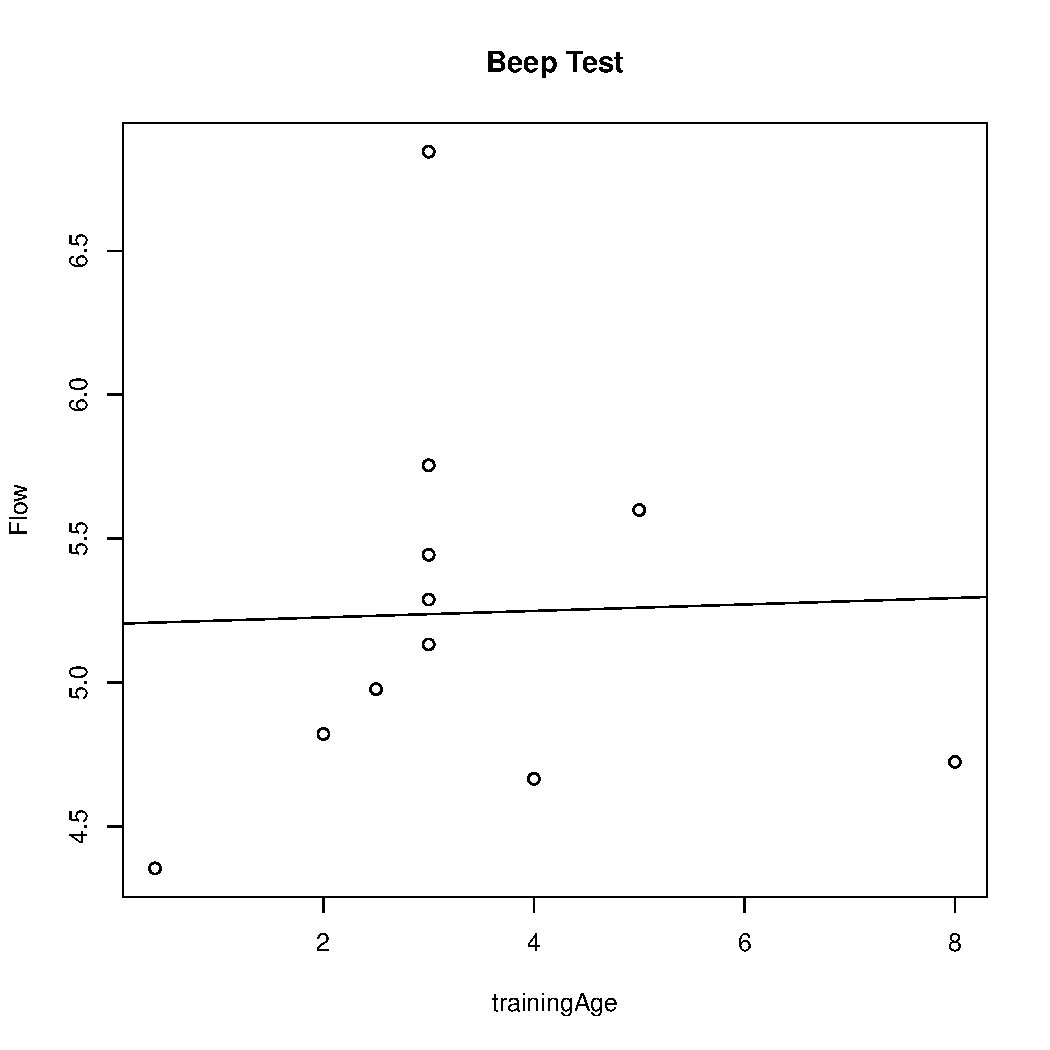
\includegraphics[scale=.2]{images/beepFlowTrainingAge.pdf}
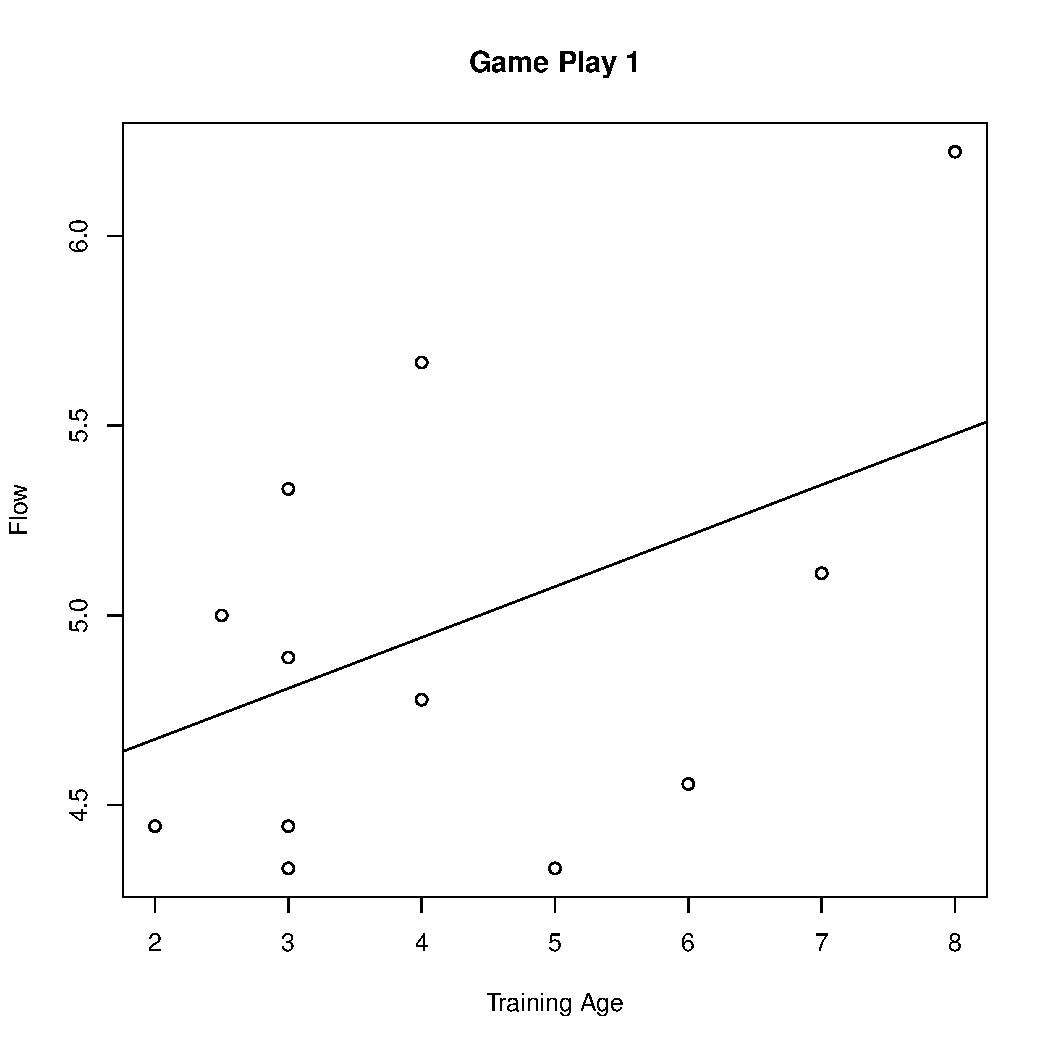
\includegraphics[scale=.2]{images/flow0109TrainingAge.pdf}
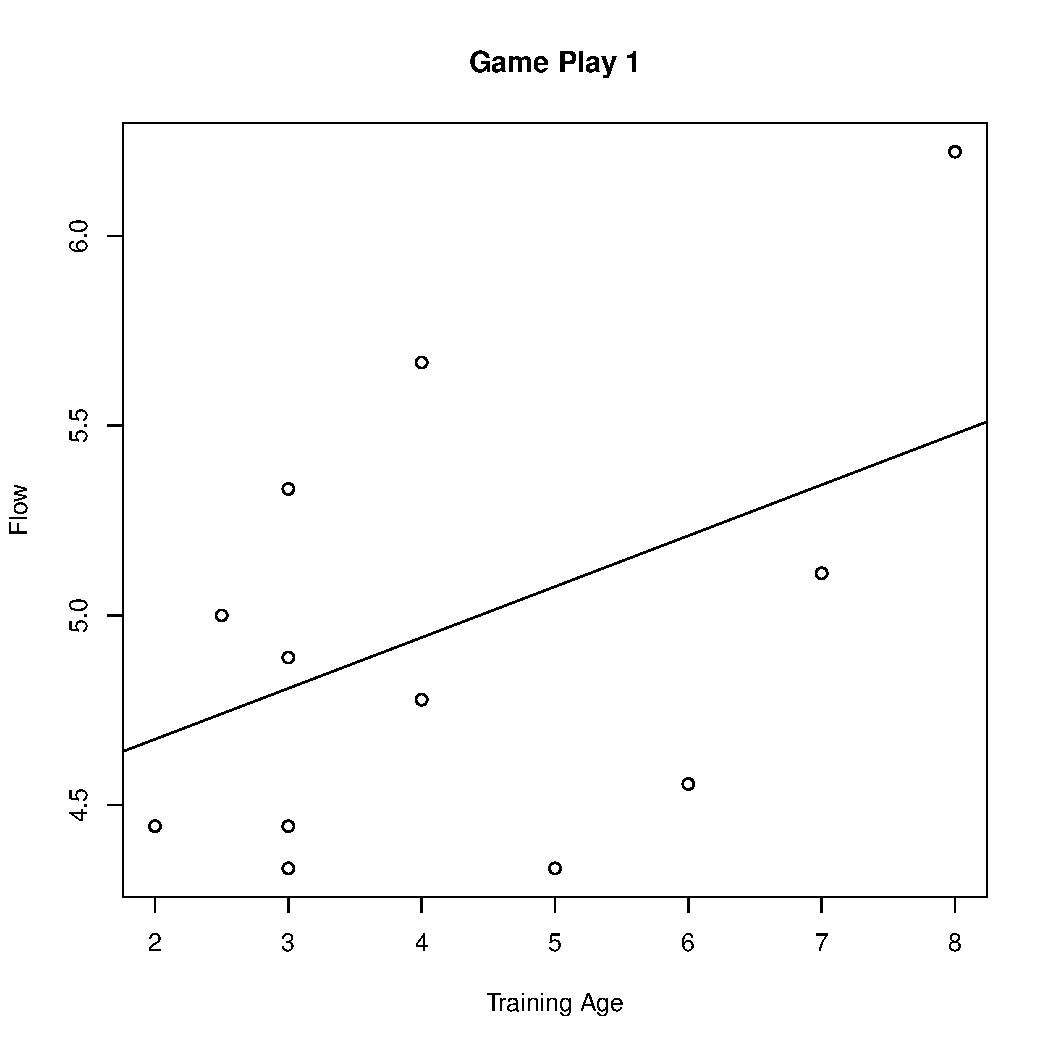
\includegraphics[scale=.2]{images/flow0109TrainingAge.pdf}
  \caption{Flow State by Training Age in three training sessions (Beep Test, Match Sim 1, Match Sim 2)}
  \label{fig:flowTrainingAge}
\end{figure}

\subsubsection{Evaluation by others and concerns about performance}
Analysis of responses to individual items of the Flow state scale revealed some contrasts worthy of further consideration.  In particular, two items relating to performance ``Just now I did not care how others would evaluate me'' (刚刚我不关心别人可能会如何评价自己) and ``Just now I did not care how I performed'' (刚刚我不关心自己的表现如何) showed noticeable variation according to training session type, as well as groupings of junior and senior athletes, and training age of athletes (see Table ~\ref{tab:postTrainingTable}).

First, responses to the survey item ``Just now I did not care how others would evaluate me'' varied according to training session and junior and senior athlete grouping.  For the Beep Test, the overall average score in response to the survey item ``Just now I did not care how others would evaluate me'' was relatively high (5.25 (1.35)).  The average for senior athletes was 5.6 (1.98), while the average for junior athletes was 5.08 (1.04).  For Match Sim 1, the overall average score in response to the same item was much lower (3.15 (1.95)). Interestingly, the average for senior athletes was higher than the mean (3.67 (1.97)), while the average for junior athletes was noticeably lower than the mean (2.71 (1.98)).  The overall average score for Match Sim 2 was 3.67 (2.19)---similar to Match Sim 1 and much lower than the Beep Test.  The average for senior athletes was 4.25 (2.12), while the average for junior athletes was 3.00 (2.34). Results for this item showed divergence between junior and senior athletes in the Match Sim sessions but not the Beep Test.

Responses to the survey item ``Just now I did not care how I performed'' revealed a similar pattern.  For the Beep Test, the overall average score in response to the survey item ``Just now I did not care how I performed'' was 4.32(1.74). The average for senior athletes was 4.55(2.39), while the average for junior athletes was 4.2(1.5).  For Match Sim 1, by contrast, the overall average response was much lower (1.92 (1.32)).  The average for senior athletes was 2.67 (1.63), while the average for junior athletes was 1.29 (.49). Similarly, for Match Sim 2, the overall average score was was 2.93 (2.22).  The average for senior athletes was 3.13 (2.22), while the average for junior athletes was 2.71 (2.21).

Scatter plots (see Figures ~\ref{fig:othersEvalPostTraining} and ~\ref{fig:indPerfPostTraining}) reveal a general trend in which more positive answers to these two items appear to correlate with higher training age, such that more experienced athletes appear to be less concerned about their own performance and the evaluation by others.



\begin{figure}[htbp]
  \centering
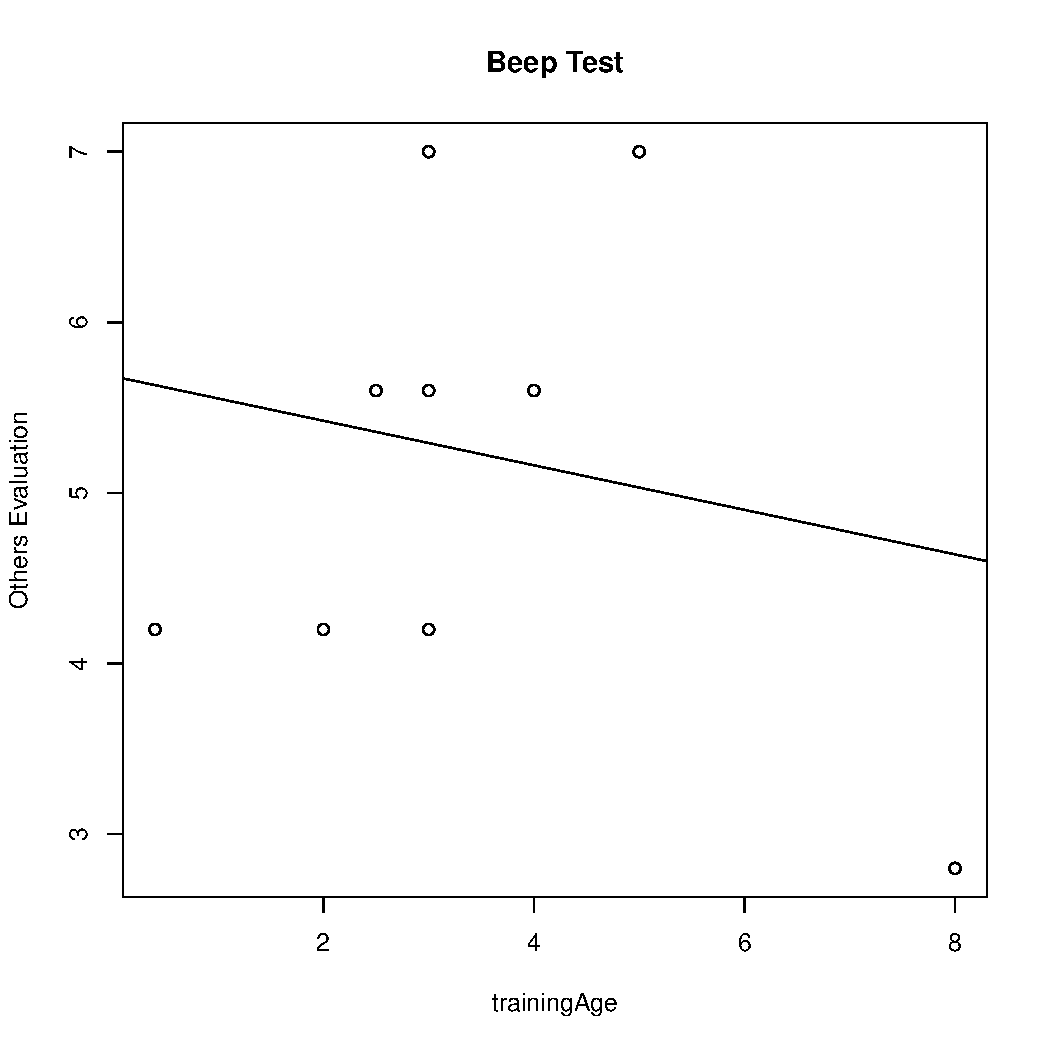
\includegraphics[scale=.2]{images/othersEvalBeepTrainingAge.pdf}
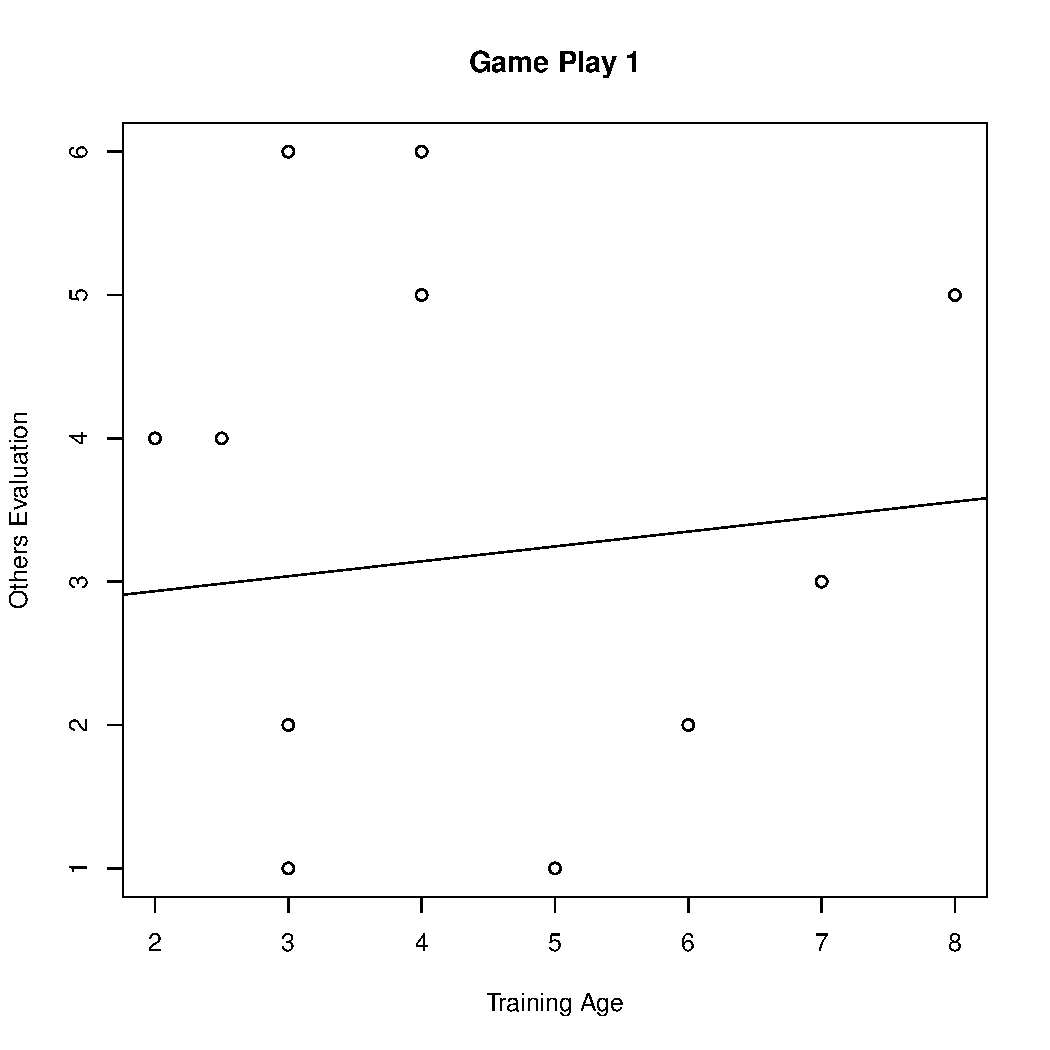
\includegraphics[scale=.2]{images/othersEval0109TrainingAge.pdf}
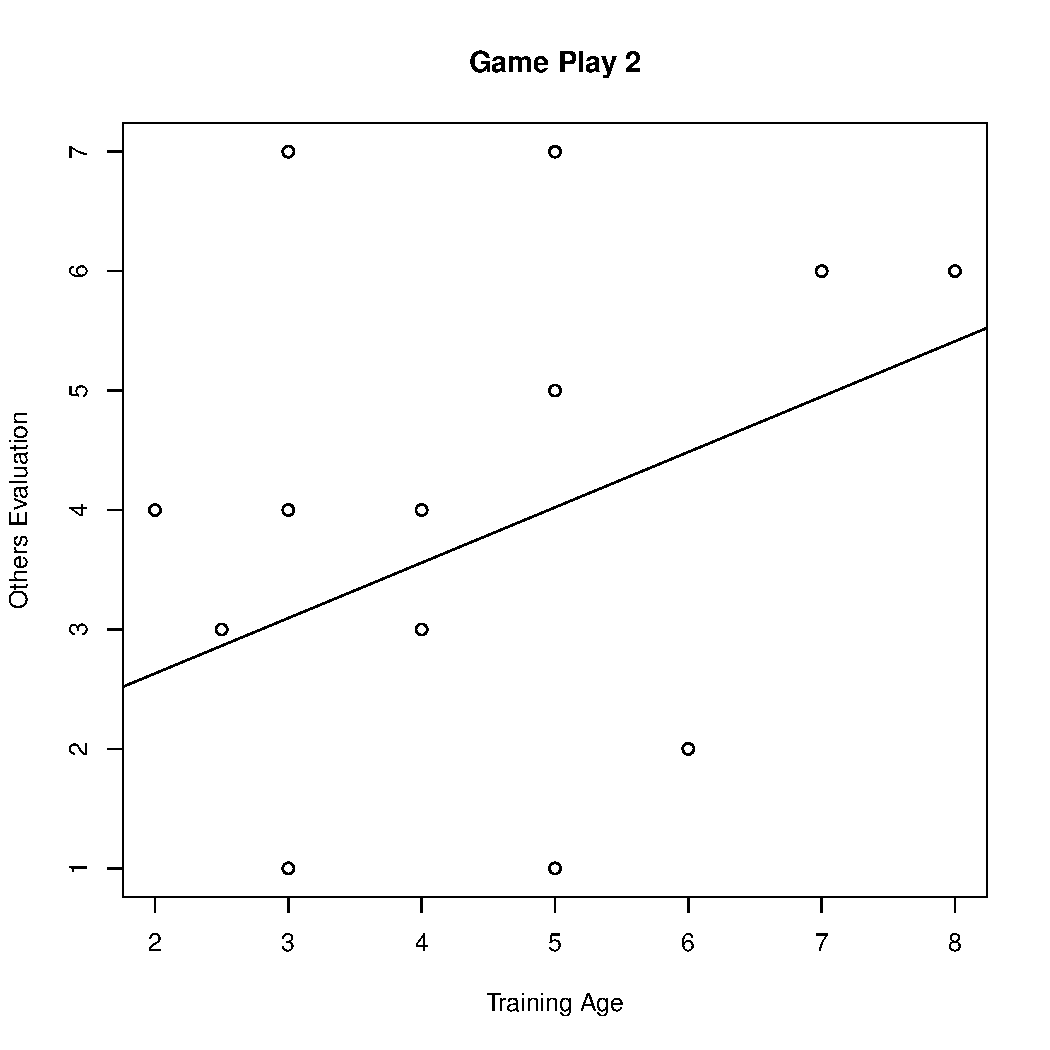
\includegraphics[scale=.2]{images/othersEval0116TrainingAge.pdf}
  \caption{Scatterplot of athlete responses to the survey item ``Just now I did not care how others would evaluate me'' according to athlete training age, for Beep Test (n = 12), Match Sim 1 (n = 16), and Match Sim 2 (n = 16)}
  \label{fig:othersEvalPostTraining}
\end{figure}


\begin{figure}[htbp]
  \centering
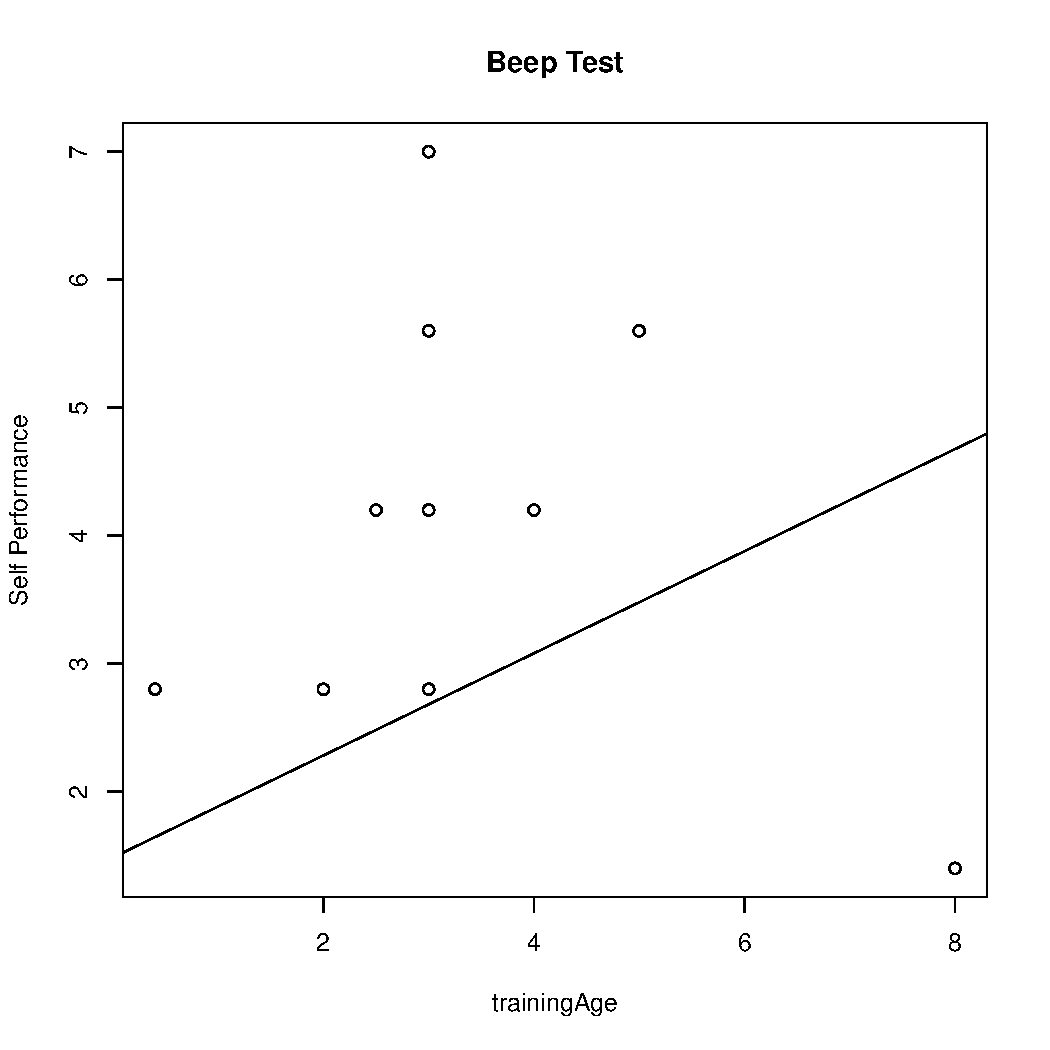
\includegraphics[scale=.2]{images/indPerfBeepTrainingAge.pdf}
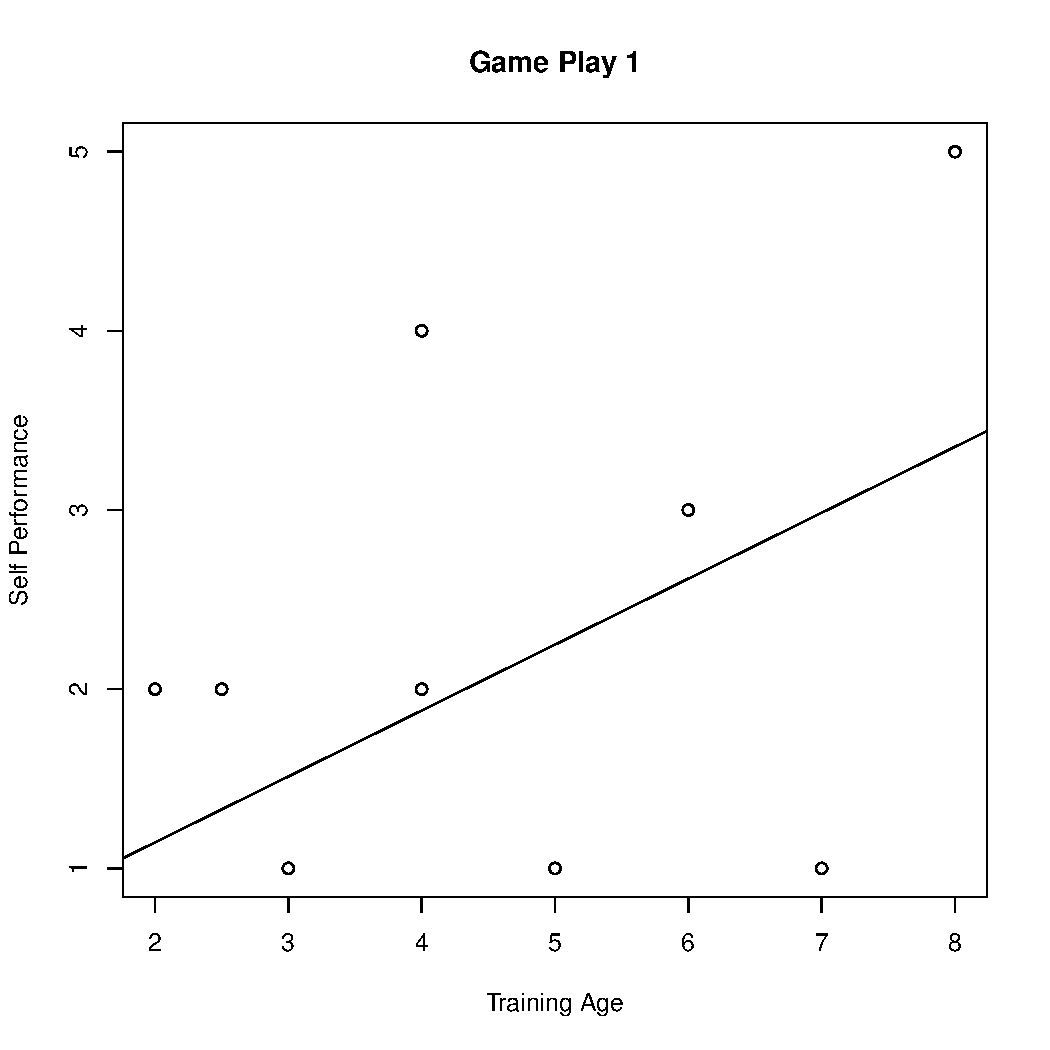
\includegraphics[scale=.2]{images/indPerf0109TrainingAge.pdf}
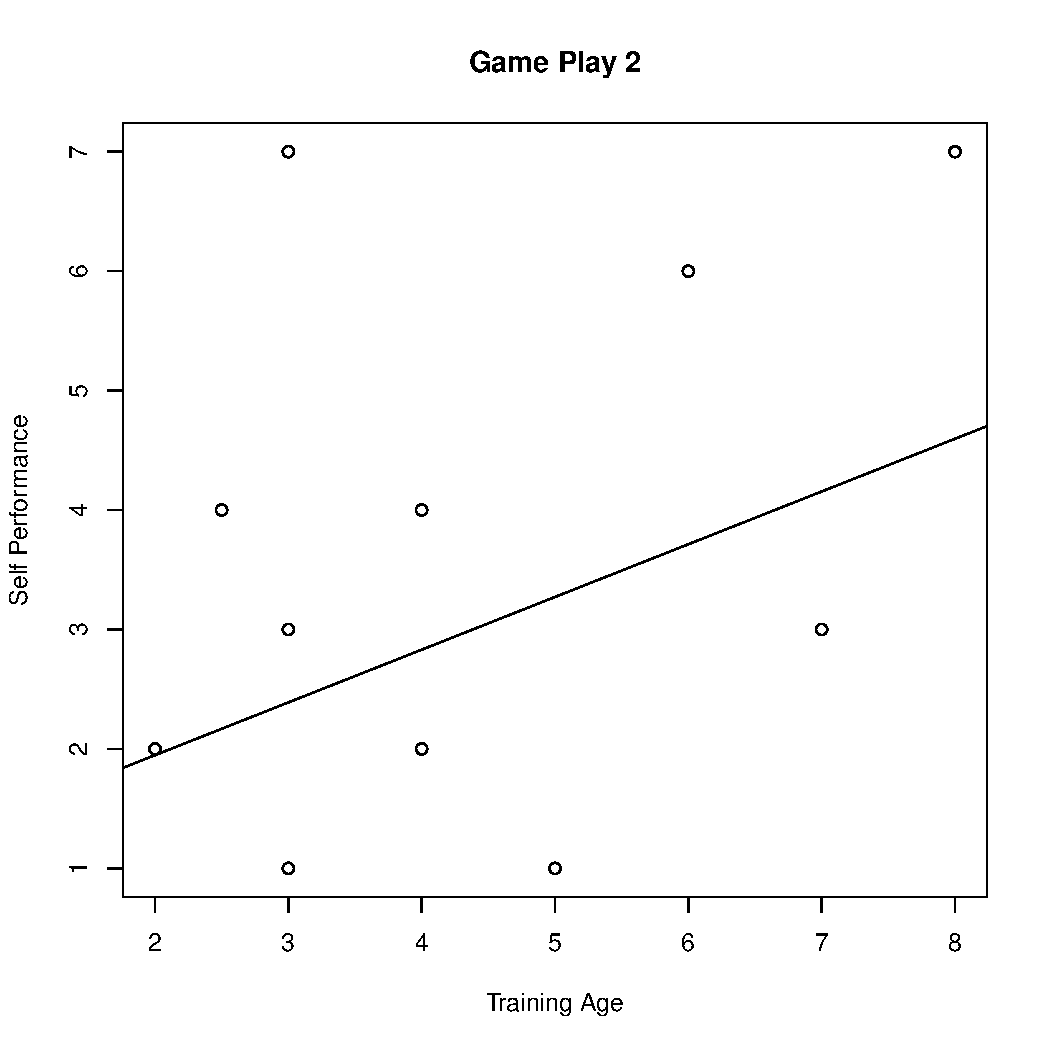
\includegraphics[scale=.2]{images/indPerf0116TrainingAge.pdf}
  \caption{Scatterplot of athlete responses to the survey item ``Just now I did not care how I performed'' according to athlete training age, for Beep Test (n = 12), Match Sim 1 (n = 16), and Match Sim 2 (n = 16)}
  \label{fig:indPerfPostTraining}
\end{figure}

These results suggest the possibility that athletes' experience of training sessions involving match-like joint action could be qualitatively different to training sessions involving fitness based tasks such as the Beep Test.  In addition, athlete experience of the on-field demands of rugby could vary according to training age and experience.

Results from these three informal post-training surveys lends some support to other sources of ethnographic data, particularly interview data, which suggests that the most salient source of challenge and stress in rugby's on-field joint action is the task of successfully coordinating behaviour with others.  While the physiological costs of rugby were experienced as a challenge, as demonstrated by athletes' collective loathing of dedicated fitness sessions, this type of stress appeared to be very different to the stress of executing joint action in-the-moment, and on the field, and as the subject of open scrutiny from the coach and more senior players. Indeed, many athletes who had transferred from other sports such as athletics insisted to me that they were well accustomed to fitness, and it was the specificity of rugby's required skills and the complexity of its joint action requirements that was the main challenge.

The generalisability of these survey results is very limited.



%In sum, these results suggest that senior athletes appear to experience lower psychological stress around performance in joint action.  In addition, the contrast between the Flow Scores for junior athletes in the Beep Test versus the training sessions indicates that the on-field demands of joint action in rugby, in addition to the rugby's physiological demands (operationalised by the Beep Test) may be the source of performance-related psychological stress.

% othersEvalBeepSeniorAvg 4.305556(1.587956)

%SURVEY RESULTS: relatively equal levels of flow overall, but higher performance related anxiety in junior athletes, particularly in the scratch matches, which required high levels of technical competence and joint action coordination.

%EXPLAIN: perception of performance in relation to social expectations of the team: joint action participation, as well as individual responsibilities (team member, self-determination)

%Senior athletes talk with more composure regarding performance, any deflect responsibility for being the agent of team performance, and show strategy regarding how to regulate energy expenditure.

%IMPORTANT: when compared to the beep test flow survey (with the senior athletes removed), reports suggest that the difference could be related to the technical complexity and scrutiny of coach and senior athletes.

%Bao Yuhan NOSTALGIA for TEAM ATMOSPHERE of the past.  Assumes role of senior, suggests that juniors are too timid, don' talk to senior players, don't let seniors know about anything, worried that senior players will tell the coach.	没有之前那会好了,那会虽然师哥师弟很厉害,但是这个气氛很严重,但是气氛好,现在没有之前气氛那么好了 。现在就是平时在一起师哥师弟很少沟通,师弟也不上我屋来,他们就觉得跟我们老的人在一起聊不下去,没天聊.  人在一起聊不下去,没天聊。有什么事不敢让我们知道,怕我们跟教练说

%Others more generous and circumspect: WW and CSC realise that it's a progression, and that individuals

%EXPLAIN: reduction of dissonance via deflection

The data presented above suggests that athletes, particularly junior athletes, attend closely to experience of performance in rugby.  Athletes report experiences of constrained awareness, vision, and thinking in on-field joint action, as well as fine-grained sensitivity
to their own performance in specific components of team and individual performance.  Performing in a way that violates their own or others's expectations appears to lead to rumination and feelings of social shame, particularly in the case of junior athletes. I also notice athletes employ strategies that serve to deflect the need to penetrate the mystery of joint action or investigate one's contribution to that mystery.  Some senior athletes, for example, appear to have developed ways of deflecting responsibility away from their own involvement in the team, and towards other targets such as the ``unruly undergraduates.''


\subsection{Positive and negative violation of expectations around performance\label{sect:expectationViolation}}

The data presented thus far emphasises on-field performance as a source of psychological stress for athletes. At the same time, I also documented evidence that athletes derived considerable joy and motivation from successful performance.  The vignette in which I describe Hongwei's journey from timid novice to exhilarated junior team member serves as an emblematic example of this phenomenon (See Chapter ~\ref{chap:theory} Section ~\ref{sect:SHW}).  In this section, I present more evidence that appears related to Hongwei's experience.

In addition to Hongwei, I noticed many other athletes gradually develop---and at times impressively deploy---a ``feel for the game'' on the training field and in competition.  My discussions with athletes in interviews confirmed the fact that athletes derived considerable motivation from the experience of discovering that they were suddenly capable of performing one aspect of rugby's diverse technical skill set.  Athletes recount with unmistakable energy and elation the moment in which their previously held expectations around individual and team performance were \textit{positively} violated.

Wang Zhengfeng offered one powerful example of athlete experience of positive violation of expectations around performance in rugby.  Wang Zhengfeng was a very talented, but still inexperienced, athlete, who had converted from athletics to rugby in 2012.  He was an athlete with outstanding physical attributes for rugby---particularly speed, agility, and strength.  Wang struggled, however, to master some of the basics of rugby's game play, such as catching, passing, and tackling. I asked Wang about his approach to the challenge of learning the skills of rugby from scratch, and he recounted the time he first discovered that he could execute a ``side step'' (a technique used by the ball carrier to evade oncoming defence):

    \begin{quote}
      JT: How do you overcome this challenge [of learning new skills in rugby]? Do you have a specific plan or way of approaching it? \\
      WZF: I imitate.  Like when I was learning how to sidestep. At the time I’d look at Brother Han (Han Xiaolong) who has a really good sidestep. I'd just watch him stepping.  Every day I'd just watch him step, and imitate him.  At the start I probably wasn't practicing it particularly well, I couldn't quite imitate it, but then after some time, I was playing touch and suddenly produced the exact action! I was so happy! Its not like it appeared at a fixed time or anything, it was like suddenly I just moved a step and it happened. And then like after I stepped once I slowly found the feeling, and then stepping became my own thing.  When you pick up new skills for the first time it feels very addictive, I get so happy, when it happens I can stay happy for a long time!
    \end{quote}

    \begin{quote}
      JT: 那你自己通过什么样的方式克服这个困难,你有计划和想法吗? \\
      WZF:模仿。就像变相一样,我当时看龙哥做的特别好,我就看他们变向,天天就看哎,模仿一下,可能开始练得不是特别好,模仿不大会,但是时间长了以后,打TOUCH的时候突然做出了这么一个动作!就特开心! 对没有固定的时间出来的,突然动了一步就出来的。比如变向突然出来之后,慢慢就找到感觉了,变相就变成自己的东西了. 做出来新的动作以后就觉得很过瘾,特别开心,能开心很长时间了!
    \end{quote}

Wang was an athlete who experienced a lot of performance-related anxiety.  Given his physical attributes and his obvious potential to be an effective rugby player (he was, for example, one of the fastest professional rugby players in China), he and the people around him (coaches and other senior athletes) held high expectations for his performance.  Often Wang felt like he didn't live up to these expectations.  When Wang did experience the feeling of perceived success in joint action, however, he felt elation that could last for ``a long time'' afterwards.  Importantly, Wang's description above indicates that the surprise of the phenomenon is an important dimension to its emotional valence.

The young hopeful athlete Yang Can, a junior athlete who also had impressive physical attributes for rugby, but was incredibly timid, gave a more low key response to a similar discussion in our interview:

    \begin{quote}
      When I first started practicing, ok, I’ll just carry the ball forward and hit it up [that was all I could do]. After that, I discovered that there are many techniques: you can fend people, you can step, you can run into a gap. There are many other actions (than just running straight towards the defence with the ball).
    \end{quote}

    \begin{quote}
      刚开始练得时候就是拿着球往前跑,撞呗,后来发现有好多技巧,也可以推人,也可以变向,也可以走空档,有很多其他动作 
    \end{quote}

While the words on the page perhaps don't quite jump out in the same way that Wang's description does, Yang Can's description of his discovery of rugby's many techniques was a bright and animated spark in an otherwise reserved interview, in which many of his responses rarely involved more than a few sentences (and often only a few word per sentence!).  His joy in describing the sensation of discovering new dimensions to his technical repertoire was clear.

It appeared that the experience of positive violations of expectations around performance can also apply to components of team (as well as individual performance).  As senior player Han explained, he only began to really enjoy rugby when he had an opportunity to coordinate with others:

\begin{quote}
    When I first started training for rugby, when I first started getting exposed to contact I was a little bit afraid, but then after I have been exposed for a longer time I became less and less afraid of contact, and then I felt more and more that as I added a few more things...like when I started to find that coordination between players when playing touch...Because I really enjoy that sort of ``two people coordinating---``pa-pa-pa'' [describing the action of coordinating movement and passes on the field in rugby] passing between players and breaking through the line'' type of feeling, I really enjoy it.
\end{quote}

\begin{quote}
  	刚开始练橄榄球的时候,刚接触对抗的时候有点害怕,但是接触的时间长了以后就越来越不怕对抗,后来越来越觉得就加了一些,会打的打TOUCH的时候相互之间有配合,因为我特别享受那种两个人配合怕怕怕配合传球最后突破的这种感觉我特别享受.
\end{quote}

In a similar vein as both Wang and Yang, Han's animated description of the feeling of ``two people coordinating (pa-pa-pa)'' elicits a positive emotional valence surrounding moments in which expectations around performance are either met or exceeded.  As discussed in Chapter ~\ref{chap:theory}, joint action poses a computational challenge to cognitive processes of prediction.   In the case of the highly interactional and unconstrained parameters of joint action in rugby, joint action is much harder to model using deliberate mental processes.  Instead, successful coordination in joint action may rely more predominantly on action-perception links and extra-neural direct coupling with the task-specific environment. It is therefore more likely that successful coordination in joint action will come as a surprise.

The fact that both positive and negative violations of expectations around performance featured prominently in both the social and emotional dimensions of athletes' experience of rugby at the Institute suggests the possible existence of an important cognitive mechanism linking joint action to processes of social bonding.  When expectations around performance are negatively violated, athletes report strong experiences of social guilt (\textit{neijiu}) and rumination on the discrepancy between perceived individual (or team) performance and the expectations around performance that they have internalised from prior experience or authoritative sources such as the coach or more senior athletes.  When these expectations are positively violated, on the other hand, athletes appear to experience a highly positive emotional response, as well as individual and collective agency.  As I will explain in the following section, it appears that when positive violations of performance expectations are specifically located in components of team performance, the result is a range of phenomena possibly relevant to processes of social bonding.

\subsubsection{Summary of results relating to perceptions of performance}
Results reported in this section suggest that the joint action demands of rugby pose a significant challenge to athletes, almost all of whom arrived at the Institute with very little understanding or familiarity with the sport.  In particular, coordinating actions with others in the moment on the field appears to arouse the most stress and anxiety, more so than individual contributions to joint action, or the fitness or injury costs of rugby (although both of these factors do appear to condition athletes' stress).  Physiological fatigue in particular appears to amplify the difficulty associated with constrained awareness and vision on the field.

Athletes appear to respond to this stress in different ways: some appear to ruminate on the perceived discrepancy between their individual contributions to joint action and expected contributions, while others instead find crafty ways to deflect and distribute responsibility for attending to this discrepancy.  These two modes of response appear to vary somewhat according to an athlete's position in the team (junior or senior) as well as factors like training age.  Individual variation in personality may also be an important factor in dictating how athletes choose to respond and behave.

In addition to the social guilt of negative violations, athletes also appear to experience positive violations of expectations surrounding individual and team performance.  As captured by the Sun Hongwei vignette, and Wang Zhenfeng's rich description of his first side step---there is something inherently rewarding (even ``addictive'') about the discovery of grasp or command in joint action.  I extrapolate more on this experience below, including the possibility that it represents the beginning of a pathway to social bonding in joint action.



\clearpage
\subsection{Team Click\label{sect:teamClick}}
In this section I outline athletes' experience of and attitudes towards coordination in joint action, particularly the phenomenology of optimal coordination or what I term team click.  Prior to beginning research,

I was also interested in the theoretical possibility that optimal performance in joint action impacted on individual and collective agency and feelings of interdependence between co-actors (see Chapter ~\ref{chap:theory} Section ~\ref{sect:novelTheory}).  In the case of optimal team performance, did athletes feel that their individual agency was blurred, extended, or enhanced by the agency of the group?  Also, did team click generate feelings of interdependence among co-actors?  Do athletes who ``click'' together perceive each other as reliable performers of their set roles and responsibilities?

In this section I present ethnographic evidence that supports the salience of the experience of team click and a relationship between team click and social processes of team membership.  The description of these processes, particularly when it derives from personal experience, is particularly animated and emotive, and often appears to contain the experience of positive violation of expectations around performance.

\subsubsection{Tacit understanding}
In semi-structured interviews I asked athletes directly about their experience of optimal coordination in joint action.  I usually began by asking athletes about the most recognisable concept team click: tacit understanding (\textit{moqi}).  In addition to his description of discovering his ability to side-step, Wang Zhengfeng also offered an animated description of the phenomenon of tacit understanding:

  \begin{quote}
    It’s really hard for me to say what it feels like.  It feels just like a fight for life or death, like you must win the match.  Normally, that sort of tacit understanding sometimes isn’t there, but then suddenly you coordinate on the field and you can form this feeling.  You haven't given much consideration as to how to play...its probably also to do with the feeling of time spent together, the few of us know each other’s characteristics, we understand each other relatively well.  Its like sidestepping, suddenly you can get that feeling of tacit understanding.
  \end{quote}

  \begin{quote}
    还真说不出来是什么感觉。就是感觉生死战一样,必须要拿下来他。那种默契平时有的时候没有,在现场上突然配合就感觉打上来了这种感觉。没有考虑太多怎么打,可能也是时间长的感觉,我们几个知道自己的特点,彼此可能比较了解,跟变相一样,突然就出来了那种默契的感觉 
  \end{quote}

Wang had just described to me his exhilarating discovery of the side-step, and so the use of the side-step to articulate an analogous phenomenon on the team level was convenient.  Nonetheless, it serves to capture the surprising and sudden sensation of successful performance in joint action.

%perhaps owing to the fact that such performance relies less on interoceptive predictive models, and more on action-perception links and direct extra-neural coupling with co-actors and other resources of the joint action environment
The fact that successful performance in joint action is often surprising could have something to do with the fact that it is often unspoken or implicit.  Senior athlete Cui Shuocheng reminisced to me about his feeling of tacit understanding with teammates in Shandong province (before he transferred to Beijing):

\begin{quote}
       Its like when you're moving the ball (passing and catching), when the ball-carrier gets there [indicating to the space in front of us in the interview room] the next person just knows what to do, like he has just one look or something and everything just moves, they both know what to do.
\end{quote}

\begin{quote}
     	当你传球和接球的时候下个人就知道做什么,好像一个眼神或者一个什么就动了,知道怎么做。
\end{quote}

Here, Cui Shuocheng draws attention to the fact that tacit understanding in joint action appears to involve an unspoken implicit dimension in which coordination is achieved without needing to articulate anything explicitly---co-actors ``just know what to do.''


\subsubsection{Flow, coherence, and control}
When I asked senior athlete Wang Wei about tacit understanding, he drew attention to the personal experience of flow, coherence, and control in joint action:

  \begin{quote}
    It feels like the ball in your hand is listening to what you say, it will go wherever you want it to go, whatever you say the ball should do, where it should run, then the ball will go there.  Its the feeling that this defender is standing there looking at you and not moving, the whole process flows like clouds or water).
  \end{quote}

  \begin{quote}
    	感觉球在手里特别听你的话,你要他去哪就去哪,你说这个球该怎么,该往哪跑,这个球奔哪去。感觉这个防守站在那看着不动。你整个过程行云流水。
  \end{quote}

Wang Wei's description of the phenomenon of optimal performance in joint action resembles evidence of flow in expert action documented by \textcite{Jackson1992}.  The experience of action is vivid, and involves both a feeling of control over action, as well as surrendering of control to the agency of the action itself.

Consistent in all of these descriptions of tacit understanding and flow reported here is the fact experiences are grounded in feelings and sensations, rather than an abstract or formal models of what optimal performance ``looks'' like (or should like).  Instead, the recognition of team click emerges suddenly, as a positive surprise and a powerful feeling.  However, as I explain below, I did notice variation in the level of granularity with which athletes described these sensations.


\subsubsection{Team atmosphere, team aura}

When I asked senior athlete Han Xiaolong to comment about optimal team performance, he drew attention to the idea of team atmosphere (\textit{qifen} 气氛), or what he insisted on distinguishing as ``team aura'' (\textit{qichang} 气场) due to the capacity of aura to delineate atmosphere located around the team:

    \begin{quote}
      Its team cohesion.  Its just team unity, the aura that arises from team unity.  Its like, look, suppose that you are an outsider, and then we are a team, and we’re all really cohesive, we are all positive, inclusive, and improving together in training, and then you can feel it from outside.  That type of feeling: that's team aura!
    \end{quote}

    \begin{quote}
      团队凝聚力。就是团结,团结起来的气场。就是,你看,你是一个外人,然后我们这是一团队,然后我们都特别团结,大家都积极向上,相互包容,相互练习进步,然后你从旁边就能感受到。那种感觉:气场! 
    \end{quote}

Han draws attention to the idea that aura is something that can be felt from both within and outside the team, from observers. Aura derives from unity: mutually reinforcing positivity, technical improvement, and inclusivity of each team member.

The importance of team atmosphere was also confirmed by athletes by virtue of their comments about its lack in the current Beijing team. Beijing local  Meng Cheng was a recent arrival to the Institute from the Chaoyang feeder school.  He commented to me on the problem with the atmosphere at the Institute:

    \begin{quote}
      When we were at Chaoyang we really had that feeling of unity, everyone in it together, for better or for worse.  As we'd improve we wouldn't focus on you was suddenly improving (more than others), we'd do more or less hand in hand.
    \\
      The atmosphere here is a bit off...its different from Chao Yang.  What I mean is that type of feeling when you drink sweet coffee and when you drink bitter coffee...its due to the relationship between junior and senior players: I feel that there is a gap.  Maybe its because of how hard it is here to play yourself into a starting position---the junior players lose a bit of hope.
    \end{quote}

    \begin{quote}
      我们在朝阳的时候特别有,大家会一起,有难同当,进步也不会说谁突然就比大家进步太多,都是基本齐头并进。

      气氛会变点味,跟朝阳不一样。变点味就是你喝甜咖啡和苦咖啡的那种感觉. 师哥师弟的关系吧,感觉有一个隔阂,因为你拿这个位置的主力觉得太难太难了,或者在队里拿一个打比赛的机会觉得太难了 ,有点绝望。
    \end{quote}

Reflections on the atmosphere---both positive and negative---were common in athletes responses in interviews.  While it was hard to articulate exactly what caused a positive (or negative atmosphere), athletes generally suggested that it had something to do with team cohesion, unity, and inclusivity.

\subsubsection{Interdependence and inter-reliability in joint action}

I also found evidence to support the idea that optimal team performance was associated with a feeling of interdependence between co-actors.  In discussions of tacit understanding and team aura above, athletes commonly refer to concepts such as team unity and team cohesion, indicating a level of coherence and alignment between co-actors.  In addition, athletes also appear to recognise their interdependence in joint action: the fact that they rely on each other to successfully perform joint action.  Hou Siqi, a member of the unruly undergraduate cohort, offered an example of the feeling of interdependence and and ``inter-reliability'' of teammates when the team clicks:

  \begin{quote}
    I have experienced [unspoken understanding] before, for example at the National Championships in Yantai (2015), or the final tournament this year in Qingdao.  I felt that the there was a particularly good team atmosphere, we were really united.  For example, if I can't make the tackle, you come in and help me make it up, if you cant make the tackle I go and help you make it.
  \end{quote}

  \begin{quote}
    有过,比如说在烟台站的全国锦标赛和最后一站青岛锦标赛,我感觉气氛特别好,特别团结。比如说我防不住的你来帮我补,你防不住我去帮你补。
  \end{quote}


Athletes often spoke in generic terms about the importance of unity due to the interdependent nature of joint action in rugby.







\subsubsection{Variation in detail and emotionality}
When I asked athletes in interviews about the experience of tacit understanding in joint action, I received responses that ranged in both level of detail as well as a level of emotionality attached to descriptions.  As a general rule, more senior athletes were able to produce more granular and detailed descriptions of what they thought were the components of team click with less emotionality attached to these descriptions.  More junior athletes, by contrast, tended to produce less detailed descriptions of coordination of joint action, and instead talked about the phenomenon in more general and emotionally charged terms.

New arrival Kang Yuzheng, for example, provided a relatively honest reponse to my questioning:

\begin{quote}
  KYZ: I have felt tacit understanding before, yes.  The feeling is really good, very flowing. \\
  JT: What is the source of this type of feeling? How do you create it? \\
  KYZ: I haven't thought about it before.
\end{quote}

\begin{quote}
  KYZ:有,感觉特别好,很流畅. \\
  JT:这种默契的来源是什么?如何创造?\\
  KYZ:没想过
\end{quote}


When I asked timid (but slightly more experienced) junior athlete Yang Can if he had ever experienced the feeling of tacit understanding in a team, he responded with the following description:

    \begin{quote}
      YC: I have before, when I was playing in that National Tournament, in that game against Liaoning Province.  Everyone was giving it their all. \\
      JT: Where do you think this type of feeling comes from? \\
      YC: (This type of commitment) comes from the heart. No matter what, you can’t let the opposition score a try, somehow you must shut them down in defence, and don’t let them run.
    \end{quote}

    \begin{quote}
      YC: 有过,在打那个全国比赛的时候。打辽宁那一场,所有人都在拼.\\
      JT: 你觉得这种很拼的感觉来源在哪?\\
      YC: 发自内心的,无论如何不能让对手达阵,怎么样也得死防,一定要防住,不让他们跑.
    \end{quote}

Yang Can's description is more a description of attitude or motivation for joint action, rather than a description of the components that allow for tacit understanding to emerge.  Both Kang and Yang's descriptions are markedly less rich and granular than those of senior athletes Wang Wei and Wang Zhengfen.

Junior athletes would often connect coordination in joint action with ideas of solidarity or unity (\textit{tuanjie} 团结) and cohesion (\textit{ningjuli} 凝聚力), without describing what they thought were the components or causes of the coordination itself.  Alternatively, some junior athletes would acknowledge that they knew of the idea of tacit understanding and other components of team click, but that their novice status meant that they had not experienced the phenomenon in rugby in particular, and were therefore unable to comment in any detail.







\subsubsection{Slippage away from on-field to off-field}

Many athletes, when asked about optimal coordination in joint action on the field, would often quickly deviate from a focus on the processes of joint action specifically, and instead move to a discussion about the team in more general, social terms.

For example, Ming Xiaokai had been training for a period of time long enough to have experienced at least some variation in the quality of team coordination.  As such, he offered a slightly more detailed description than some of his more junior counterparts:

    \begin{quote}
        MXK: Tacit understanding is definitely there, but its relatively rare. But when you’re up against it in a match you feel very united, especially when sometimes you take the lead again. \\
        JT: What do you think the source of this feeling is?  How do you achieve this sort of result? \\
        MXK: No matter whether its on-field things do do with training, or off field things, like some interaction off the field, some communication, when its a bit of fun, when we're all relatively good friends, you know?  When its like this, I feel like I would like to try a bit harder, share more things with others, that type of feeling.  If my teammate gets tackled I'll get really angry and want to help them.
    \end{quote}

    \begin{quote}
        MXK: 默契肯定是有的,但是比较少,但是打逆风球的时候会特别团结,有时候会反超. \\
        JT: 你觉得这个感觉的来源是什么?如何才能得到这种效果?\\
        MXK: 不光是训练场上的东西,场下的东西,场下的一些交流,一些沟通,比较好玩,比较好朋友吧,我感觉天天场上做的时候感觉想多努力一分,多分享一些东西,这种感觉。他们要是被扑搂了,也会很有气儿,会想去帮助他们。 
    \end{quote}

Ming Xiaokai emphasises the role of communication and interaction on and off the field in producing the feeling of tacit understanding.  Despite taking the liberty to explore the concept in more detail than Yang Can, Ming Xiaokai also ends up settling on a general feeling rather than particular details.  In this instance, he emphasises the feeling of solidarity and interdependence with a teammate.

Lu Zhongsheng (a.k.a. ``Big Mouth Monkey'', see Chapter ~\ref{chap:ethnoField} Section ~\ref{sect:savingFaceJointAction}) was a gregarious senior athlete who was very talkative in our interview.  When I asked him about how to achieve tacit understanding, he replied with much more conviction than his more junior athletes.  However, his convictions soon led him to drift away from an analysis of the particulars of joint action, and instead towards descriptions of solidarity and emotional closeness with teammates:

    \begin{quote}
      First of all, you have to have a common direction and goal.  For example, which team are we going to take down today---everyone has this ``must win'' conviction in their mind.  Everyone works together; no abandoning each other and no giving up, most importantly when you’re behind (in a match) you can’t give up, there’s still hope, as long as the time is not up there is still hope.  We shoulder the pressure and are determined to prove ourselves.  It's the presence of that real feeling that ``all for one and one for all''.  And then that feeling of everyone crying together is great! Because we've endured such agony...
    \end{quote}

    \begin{quote}
      首先是大家有一个共同的方向和目标,比如说我们今天要把哪个队拿下,大家每个人的脑子都有这个必胜的决心,大家一起努力,不抛弃不放弃,最重要的是及时落后了也不能放弃,我们还有希望,时间还没到我们就还有希望。背负压力,我们一定要做好,就像我们要证明自己。真正的在场上每个人都做到那种“人人为我我为人人”的感觉,然后比完赛大家都一起哭了那种感觉特别棒!很痛苦我们都吃的...
    \end{quote}

When I asked junior athlete Meng Cheng to explain how tacit understanding and atmosphere are generated in a team, offered a very emotive response:

      \begin{quote}
        If we want to play, we do it together, and usually there’s nothing we can’t say to each other.  For example every week a few of us all drink and eat a bit and have a chat.  I think this is very important, because if you have a drink and a meal and talk a bit of shit you feel relatively...you generate that feeling you know? Like when you’re drinking together and you feel particularly intimate, really close.  Besides that then its also when you’re doing fitness and can’t keep up and the coach is going to punish you, and so whoever can’t go on you give him a hand and pull him along.  Everyone has the same goal and is motivated.
      \end{quote}

      \begin{quote}
        大家要玩一起玩,平时无话不说。比如每周咋们几个大家喝点(酒)吃点聊聊天。我感觉这个很重要,因为你喝点吃点吹点牛感觉是比较。。。你来这个感觉吗?比如说喝的时候感觉特别亲密,特别亲。剩下就是体能训练的时候跟不上教练要罚的时候一起挨罚,谁跑不动了就拉一把。大家目标一致,都有上进心。 
      \end{quote}

Once again, like Xiaokai and Big Mouth Lu, Meng Cheng quickly deviated from describing optimal performance in joint action to describing social processes off the field.  The automatic slippage between talking about tacit understanding in joint action and team processes off the field indicated to me that, in this context at least, that team click and social bonding were importantly intertwined.  A core reason for the slippage away from talking about specifics of joint action seems to be related to the inaccessibility of joint action to conscious reflection.

More senior athletes tended to stick to a more detailed and granular description of what they considered to be the experience of optimal joint action. Interestingly, however, senior athletes would also easily slip off the topic of joint action.  But instead of venturing towards notions of team solidarity and unity, they tended to problematise the lack of these components in the current team, and would point to various rationales for why this was the case.  For example, after his nostalgic recount of team click in the Shandong team, Cui Shuocheng then immediately tranferred into an analysis of why click is less present in Beijing: ``I feel that in Beijing (we) play too singularly, its just that type of pass the ball, pass the ball''  (感觉在北京打得太单一,就是传球传球之类的).

Senior athlete and coach Lu Peng, always keen to problematise the athletes below him, explained why he thought that the current Beijing team lacked tacit understanding in joint action.  When I asked him if there was any click in the team currently, he replied:

      \begin{quote}
        No, its very rare.  Not like it was with us before (before 2013), because when we were like that...back then, the status of the Beijing team in China was such that if you were in the starting team for Beijing, it was very hard to experience any disdain.  At that time through our own efforts we would understand that sort of concept from of a ``national team.'' And when we'd go out to compete we'd work hard.  Now they (the more junior Beijing athletes) wouldn't come and find senior athletes to discuss these sorts of things.  They're thinking about their own little things every day.  They won't think about it, and also they won't go and do it.  They skimp their way through training.  \\

        It is very important thing for athletes to be--- my former coach used to say this word, I don't know how to say it in English, in China we'd say this athlete has a strong ``animal intelligence.'' Ok, I'll try to explain it to you: animal intelligence is talking about, well first we are all primates right?  And primates are really smart!  So this so called animal intelligence, in the case of rugby, is that on the field you have incredible creativity: you can do things that others don't expect.  This is the idea of animal intelligence in an athlete.  And you can do it often, inconceivable things, when you're extremely intelligent on the field. This is animal intelligence.
      \end{quote}

      \begin{quote}
        没有,很少。不会像以前我们那样。因为我们那样的时候,以前我们北京队在中国的情况下,如果你是主力队员的话,你很难体会含怒。那时候是我们通过自己的努力把国家队的那种理念都看懂了,前后我们出去主要是努力。现在他们不会去跟老的聊这些。天天在想自己的小事情。他不会去想,而且也不会去做。训练的时候敷衍了事。球员很重要一点就是,教练曾经说过一句话,我不知道英文怎么讲,在中国中文讲是这个球员很有灵性! ...我试一下给你解释啊:灵性就是说,咱们单人都是灵长动物是吧?就是特别聪明的!就是所谓的灵性就是对橄榄球的话就是, 在场上你有很好的创造力:别人想不到的你能做出来,就是灵性。 经常能做出来。 想不到的东西,特别聪明,特别灵性.
      \end{quote}

I went on to probe as to why younger athletes did not display this mysterious ``animal intelligence'' in rugby:

\begin{quote}
      JT: Why do you think the young athletes don't have this intelligence, is it because they're not motivated? \\
      LP: That's right, its a problem with the environment they're in, there is no competitiveness, no motivation.  At that time we were very competitive and so we were motivated.
\end{quote}

\begin{quote}
      JT: 那你觉得年轻队员不做这个是因为没动力?\\
      LP: 对,环境问题嘛、没有竞争力,没有动力。我们那时候就是很有竞争力,有动力。
\end{quote}

Lu's exegesis of the sources of team click was brimming with nostalgia for a former era of the Beijing team.  In this imagined previous era,  athletes developed a level of mastery on the field due to an environment in which athletes where competing viciously with each other for a spot in the team.  Without the same level of motivation, the current squad of athletes did not develop that mysterious quality of animal intelligence.  The precise causal pathways between social competition and on-field performance in joint action are poorly understood, and athletes lack direct and objective access to the mechanisms of joint action.  Nonetheless, Lu is in a position of authority in which he is able to offer an explanation for team performance.  Animal intelligence thus offers Lu a vehicle through which to explain the sources of optimal performance and justify its current lack in the Beijing Team.

When I asked him about the reason for a lack on on-field click in joint action in the Beijing team, senior athlete Ma Haitao utilised a cultural (environmental) explanation to account for the team's issues with on-field performance:

\begin{quote}
  MHT: Chinese people's sense of initiative (conscientiousness) is very poor.\\
  JT: Why do you think that is the case, really? What is the reason [for Chinese people's poor sense of initiative]? \\ MHT: Environmental factors, environmental influence.  Like you all (Westerners) from a young age in your environment you think its just has to be done like this.  Our environment isn’t like that.  First, (in a group situation) you (as a Westerner) will think ``we are all teammates,'' and your team all think that this principle is very important.  But we all think ``it doesn’t matter, I can just go with the flow and that’s enough.''  But you are not like that, you are like ``this is just how it must be done.'' Just like what we were talking about in the gym, about your personal ``disposition'': you said you need to get up in the morning and feel like you're being productive... China also has this disposition, its always ``have a look first'' (before committing to anything)...
\end{quote}

\begin{quote}
  MHT: 我们中国人自觉性很差. \\
  JT: 为什么?到底?原因在哪?\\
  MHT: 环境因素,环境影响。像你们,从小你们环境影响觉得就该是这样。我们环境影响不是这样。一是认为``你们是队友'',你们队都觉得这个很重要!但是我们觉得 ``无所谓,我变通一下就可以了''. 但是你们就不是,你们是 ``他就应该是这样了''就像我们在健身房聊天说那个 ``形势'', 早上起来要干啥,中国也有一口, 他就是总的形势是  ``看一下''...
\end{quote}

Problematising Chinese culture, by contrasting it with a valorisation of ``Western'' alternatives, is a common trope in contemporary Chinese social discourse, with strong historical roots \citep{Liu1995a}.  Much like Lu's use of animal intelligence, Ma's appeal to cultural variation (in this case between China and the West) as an explanation for performance outcomes in joint action serves as a convenient vehicle to account for what are, in reality, complex mechanisms and coordination dynamics in joint action to which athletes have very little direct access.

Senior athlete Pan Qiyu also critiqued the Chinese sport ``system'' (\textit{tizhi} 体制), drawing attention to the fact that the Chinese competitive sport system is inherently problematic for fostering effective on-field coordination:

\begin{quote}
  Take Chinese football.  If you’re talking about competitive sport system in China, the Chinese football team can barely beat a random student team. Its a complete mess! There’s no thinking in competitive sport, nothing in the brain, no innovation (to use a foreign way of speaking), there is no will to build emotional connection, coordination, or tacit understanding between teammates, and so it leads to this type of feeling at the moment.  So that's why I think Basketball, football, rugby must all develop as school sports, like they did in America, Japan and also Europe. They all developed their sports in schools. From a young age, [students] first develop interpersonal skills of communication and team awareness, and I think this is really great.  The Chinese sport system is missing this.
\end{quote}

\begin{quote}
  我觉得这个中国足球,竞技体育,连个学生把子都踢不过,天天战乱!,所以竞技体育,人的脑袋没有东西,没有创造力(就是用外国的说法),队员之前没有感情,没有配合,没有默契的意志,导致这种感觉。所以我还是觉得什么篮球,足球,橄榄球必须走校园体育开展。应该像美国日本包括欧洲,都是在校园开始开展,从小开展,一是培养人与人之间的沟通和团队意识,我觉得这个比较好。中国体育体制就却这个
\end{quote}

When I then went on to ask Pan about the feeling of tacit understanding and team click, he naturally drew upon his critique of what was lacking in the Chinese sports system to describe what is important to optimal coordination:

  \begin{quote}
    PQY: I have experienced the feeling of tacit understanding, yes. I've had harmonious times and unharmonious times. When I was in Dandong (Liaoning Province) that team was relatively harmonious.  The seven of us on the field I felt were pretty unified, I felt that that kind of atmosphere was really good. \\
    JT: What do you think is the source of that feeling? \\
    PQY: Every individual is inclusive and positive, and accommodating of each other. Every individual has weaknesses, but then everyone is accommodating of the weaknesses on the field, I feel that its better like that, its more motivating, it makes people...
  \end{quote}

  \begin{quote}
    PQY:有过,有过和谐的时候也有不和谐的时候,我在丹东的时候那支团队比较和谐,我们场上的那七个人我感觉是比较团结,感觉那种氛围感觉比较好 \\
    JT: 你觉得这种感觉的来源是什么?\\
    PQY: 每个人很包容和积极,大家都很互相包容。 每个人都有缺点,但是每个人都包容每个人的缺点在场上, 我感觉这个比较好,比较动力,比较能让人。。。
  \end{quote}

Like many other athletes I interviewed who attempted to articulate the factors behind the click of joint action, Pan also failed to put his finger directly on what team click was, and how it is most effectively generated.

\subsubsection{Summary of results for feelings of team click}

The excerpts discussed above contain evidence of a range of salient components to optimal on-field coordination.  Athletes cite experiences of tacit understanding, flow and control of action, team atmosphere, a sense of interdependence with others, and a level of reliability between co-actors to produce desired outcomes in joint action.  Importantly, these experiences are often surprising, exhilarating, and autotelic \citep{Csikszentmihalyi1990}.

I notice variation in the detail and emotionality of descriptions around flow. As a general trend, more junior athletes appeared to be less detailed and more emotional, connecting team click to emotional solidarity and togetherness.  More senior athletes, by contrast, went into more detail and communicated less overt emotion about the team.  Both junior and senior athletes were prone to slippage between talk of on-field coordination and talk of off-field social dynamics, and athletes drew upon environmental, cultural, and zoological (animal intelligence?).

Athletes' explanations for optimal on-field coordination revealed that athletes do not have direct access to the causal mechanisms of joint action, and instead draw upon reflections about the broader social processes and dynamics of the team.  The extracts included above offer evidence that athletes draw a link between on-field coordination and social processes of group formation.  Tacit understanding derives from and produces team cohesion, while lack of competition, motivation, or conscientiousness leads to a lack of on-field ``animal intelligence.''  While more senior athletes were able to produce elaborate exegesis for processes of joint action, more junior athletes tended to immediately conflate team click with team cohesion, perhaps owing to their lack of fine-grained personal experience of on-field joint action.  Senior athletes' explanations also functioned to distract attention away from individual responsibility for coordination in joint action.
















%Lu Zhongsheng:
% LACK of CLICK in BJ: “No one wants to mention this…but this, I think this is a big problem for the Beijing team at the moment, everyone is very selfish.  There are only a few people who are willing to instruct how to do it (how to play rugby), the rest all think "you are you, I am me, whatever I want to do today don't interfere with me, you don't need to think about me, I don't need to think about you.  This play, for example a simple draw and pass,  the easiest thing is to pass the ball and the play is made, but he just doesn't want to give it to him, he wants to do it himself... and then he'll come up to you and blame you and say "why weren't you faster to support me?" This is the sort of... this is the team at the moment.  You look at the atmosphere in contact at the moment, you can see, he doesn't want to line up against him, he doesn't want to line up against him...why then? Its not because they are afraid, actually.  Its because whatever I do on the field, he is going to have something to say about it off the field, he'll be angry and giving me the look.  Recently this I particularly put off by this, its a big problem."	: 大家都不愿意提起的事情。。。这是北京队现在的一个我觉得是一个非常大的问题,大家都很自私。只有这两个人愿意去告诉我们该怎么做,其他人都是觉得“你是你,我是我,我今天想怎么做你不要干涉我,你不需要为我考虑,我也不需要为你考虑”。这个球,定人传球让他打就行,但是我就不想给你,我就想自己干,别人过来还怪你说“你怎么没有快点过来支援我呢?”有这种。。这是这个队伍现在,你看现在对我打对抗的气氛,你就可以看出,他也不想打他,他也不想打他,为什么呢?不是害怕,其实。我在场上打,我在场下他还得和我说话,急眼了,生气了。我最近特别讨厌这个。是个很大的问题。 























\clearpage
\subsection{Group Membership\label{sect:groupMembership}}

It was clear from my ethnographic observations that despite the explicit utilitarian incentives for life-course opportunities that drove individuals' adherence to rugby at the Institute, the Beijing men's team rich psychological resources of belonging to athletes, coaches, and officials alike.  By virtue of their membership to the team, athletes found friendship, emotional support, guidance, and, importantly, social identity.  In the previous section, evidence suggests that while the details of on-field joint action are difficult to explicitly articulate, the feeling of tacit understanding between athletes on the field may offer a visceral grounding for psychosocial processes of affiliation and trust.

Lian Jianxiang was a young trialist from the Coach Zhu era of the team who who was branded by Wang Wei as an athlete concerned primarily with the utilitarian motive of finding his way in to university.  Lian Jianxiang left the team in February 2016, shortly after Zhu left, and after Lian himself had endured a series of injury hardships.  18 months later in August 2017 I ran into Lian on the sidelines of the National Games in Tianjin. Lian was in Tianjin to support the Beijing men's and women's teams.  He wore his Beijing Team apparel and banged loudly on the supporter drum all weekend in support of his former team, leading group chants of ``Go Beijing! Go Beijing!''.  All of the utilitarian benefits that adherence to the program offered had all but disappeared for Lian, yet his identification with and devotion to the team remained very clear.

As I discuss in more detail below, when I asked athletes to expand on their thoughts around group membership, three core categories emerged from responses.  Athletes tended talked about: 1) emotional support derived from group membership, 2) the importance of a sense of shared goal with teammates, and 3) the social identity that they derived from adherence to rugby.


  \subsubsection{Emotional support\label{sect:emoSupport}}

Interview data suggest that athletes experienced a strong emotional connection to their teammates and to the team.  As Meng Cheng explained: ``you generate that feeling you know? ...you feel particularly intimate, really close'' (see above in Section ~\ref{sect:teamClick}).  Lu Zhongsheng recounted a similar phenomenon: ``It's the presence of that real feeling that `all for one and one for all'.  And then that feeling of everyone crying together is great! Because we've endured such agony...'' (Section ~\ref{sect:teamClick}).  Even the intense critiques of the state of the team launched by the likes of Lu Peng and others can also be interpreted, in one sense, as an indication of emotional attachment to the team.  Over the course of my fieldwork, Lu spend many hours in my room talking to me about rugby and the situation with the team.  A less invested individual would conceivably not spend the time and energy on intense examination of the problems with the Beijing team.  In his own way, Lu was committed emotionally to the team and to rugby.

Athletes produced many versions of the same idea of solidarity through group membership, all of which entailed an element of emotional support. For example, when I asked him about his experience of group membership, junior athlete Yang Can explained:

    \begin{quote}
      Because rugby is a team sport, you know. We’re all brothers, it's the same as fighting, we’re born brothers and we’ll die as brothers you know, like a family, all together, thinking about how to share the responsibility. Its really good...I had never experienced this feeling before.  At that time at primary school there weren’t any rules, you’d just muck around or at the end of school just leave straight away, there wasn’t this type of feeling there.
    \end{quote}

    \begin{quote}
      因为橄榄球就是团体项目嘛,都是兄弟,像打架一样,出生入死得兄弟嘛,就跟一家人一样,互相,多替别人考虑分担,挺好的...没有过这种感觉,那时候小学没有什么规矩的,直接玩或者放学就大直接走了走了,没这种感觉
    \end{quote}

As noted above, Yang Can was an extremely timid and reserved individual in public team settings, and the interview that I conducted with him was dominated by very brief responses. Just like his flourish when describing the exhilaration learning the new skills of rugby (see Section ~\ref{sect:expectationViolation} above), here Yang Can also came to life when talking about his experience of team membership.  This passage revealed to me that he harboured a strong identification with the team, which was underwritten by a strong emotionality.

At the time that I interviewed him (in January 2016), Guo Junping was one of the team's newest trialists.  Guo was from Fujian province in China's south, and coach Zhu had organised for Guo to come to Beijing following a recent scouting trip that Zhu took to Fujian.  Guo had just finished high school, and he (and his parents) were no doubt interested in opportunities to attend university.  He had never played rugby before, and had only a brief background in athletics before arriving.  When I asked him about his views on rugby, after only a few weeks of training in Beijing, he responded:

  \begin{quote}
      I really like this sport.  I liked it at the time that Huang introduced it to me [his high school coach in Fujian]. Its not like athletics.  Athletics is an individual sport, I prefer teams.  There is more passion, there are mates playing together.  Its like playing computer games, I’m happy when there are people to play together with, it's a team sport.
  \end{quote}

  \begin{quote}
    	挺喜欢这个项目。当时黄老师介绍时候我就喜欢,跟田径不一样,田径是单人项目,我比较喜欢团队,比较有激情,有伙伴一起玩,跟玩游戏一样,有人跟你一起玩就开心,团体项目。
  \end{quote}

In a similar fashion to Yang Can, the emotionality in Guo Junping's explanation was strong and powerful compared to his other responses in the interview.  Guo's utilisation of computer games as an analogy for the team sport of rugby was not accidental. I soon came to realise that computer games, particularly multi-player interactional games involving team membership and intergroup competition,  were a central part of athletes' lives (for an extended discussion of the role of computer games in athlete's lives, see Appendix ~\ref{app6:ethnoResults} Section ~\ref{sect:computerGames}).

Over time I noticed that emotional support was often expressed in association with the adversity or stress of joint action in rugby.
As senior athlete Pan Qiyu---ever-eloquent in his articulations---explained to me:

    \begin{quote}
      I think that through rugby you can meet friends, you can train your awareness of social unity, and this sort of awareness of hard work, toughness, and struggle.  I think all these things are very...for example every time you run fitness, at the time it is incredibly tough, but once you’ve finished your mood is extremely cheerful, even though you are very exhausted, its still really happy.
    \end{quote}

    \begin{quote}
      我觉得通过橄榄球能交朋友,能锻炼自己的团结的这种意识,刻苦,艰苦,奋斗的这种意识,我觉得这些都很。。。比如说每次跑体能啊,当时特别辛苦,跑完之后心情非常愉快,虽然跑得很累,但是跑下去很愉快的感觉。 
    \end{quote}

Similarly, unruly undergrad Ming Xiaokai expressed his experience of team membership:

    \begin{quote}
      Friendship: the feeling of playing alongside really good friends, good mates, scoring a try together, winning by one score after the scores are level all game, its especially, especially joyous, very exciting.  That's it really, when things are really tough, and when we all come in and put our hands on the ball, I’m really happy.
    \end{quote}

    \begin{quote}
       友情。和特别特别好的朋友,特别特别好的哥们儿,一起打球的感觉,一起达阵,平分赢一个球一起赢的那种激动,特别特别开心,很激动。主要就这些,特别困难的时候,打发成球,特别开心.
    \end{quote}

These interview excerpts are strong indicators that processes of group membership associated with the rugby team at the Institute offer athletes a level of emotional support.  My ethnographic observations (beyond these interview data) confirm that members of the Beijing team developed strong bonds of friendship with their teammates.  Athletes trained, ate, slept, and bathed together (in communal bathrooms).  Indeed, some athletes spent the majority of their formative high school, university, and young-adult years together.

\myparagraph{Saturday night hot pot}
The details of the Saturday night I ate hot pot in Han's dormitory room (along with Cui Shuocheng, Wang Zhenfeng, and Meng Cheng) captured the camaraderie among the group (see Chapter ~\ref{chap:ethnoField} ~\ref{sect:allComplicated}).  The setting in which we ate was itself very intimate.  Some sat with Han on Han's bed, and the rest of us sat on small stools around a small table in the middle of the dorm room.  The communal pot sat atop a portable electric stove element, and Meng Cheng, the youngest in the group, was tasked with cooking the meat and vegetables in the boiling broth.  The rest of us chatted away, dipping our chopsticks into the pot occasionally to fish out some food.  We covered a range of topics, including the topics mentioned in the previous chapter.  Every so often, Cui Shuocheng would dispense a small portion of Beijing ``\textit{Niulanshan}'' (牛栏山) rice wine to each of us and we would chink glasses.  Food and drink enjoyed in this manner was an age-old Beijing pastime. It was Saturday evening at the end of a long week of training, and this was an appropriate time for socialising as friends.

One topic that dominated conversation for a large portion of the evening was that of junior athlete Zhang Bo's love life.  As it turned out, that evening Zhang Bo was in the process of ``expressing his heart'' (\textit{biaobai xinji} 表白心迹) to the woman that he had been recently seeing.  At the time of writing, the act of using grand gestures to express one's heart romantically to another was very popular among China's youth.  Meng Cheng explained that after training finished at lunch time, Zhang Bo and his friends (predominantly junior athletes, including Meng Cheng, Bao Yuhan, Jiang Wei, Ming Xiaokai, Fang Chao, and Yang Can) had been helping Zhang Bo prepare an elaborate evening of activities.  Meng Cheng showed me a photo of the climax to the evening: a private Karaoke room lit with 520 (520 was the colloquial numerical stand-in for ``I love you'' 我爱你), little candles arranged in the characters of Zhang Bo's love interest's name, and red rose petals scattered around the room.  This arrangement and other organisation had taken Zhang Bo and his friends the entire afternoon to execute, and Meng Cheng was visibly excited about being part of the preparations, as were the rest of us in the room listening to Meng recount his efforts.   The devotion that Meng Cheng and others showed to Zhang Bo by helping him with this elaborate activity was an obvious signal of genuine friendship, underwritten by an emotional bond.

\myparagraph{Beijing 10s Tournament}
Throughout my time with the Beijing team I watched them play in a number of rugby tournaments, and these experiences invariably exposed an obvious level of emotional support and commitment between group members.  Early in my first stint of research I went with the team to the annual Beijing 10s rugby tournament, which was attended by the Beijing Team and the three other expat rugby clubs based in Beijing.  In the final match of the day, the beijing team were playing the Beijing Devils 2nd Team.  Early in the first half, tensions began to simmer between the two teams due to a late tackle made on a Beijing player by a Beijing Devils player.  As soon as the Beijing player took offence to the late tackle, it sparked a disruption in play, as other players from both teams came in to support their teammate.  This scuffle drew immediate and instinctual response from the sidelines, and a few of the reserves on the Beijing team dropped their water bottles and began to run onto the pitch in solidarity with their teammates.  My instinctual response was to reprimand the Beijing athletes and tell them that according to the norms of rugby, it was inappropriate to storm the field in these situations---this was something that the referees and players could sort out among themselves on the field.  Play continued, but tensions between the two sides persisted for the duration of the match.

With only one minute to play, the scores were locked at 10 point each.  Amazingly for Beijing, senior athlete Wei Wenxin pounced on possession of the ball and beat a series of defenders to score a try under the posts to win the match.  Wenxin was elated, as were his teammates both on the field and on the sideline.  As soon as he put the ball down over the try-line, he turned around to the Beijing Devils team chasing after him and screamed out (in English) ``Fuck!'' while making a grand and aggressive upper-cut movement pointing his index finger in to the air to signal triumph.  Wenxin was obviously elated with victory, as were his teammates. And while most of his teammates thought that his choice of word was a little bit crass (I think he may have been trying to express a more celebratory ``Fuck yeah!'') they all seemed to resonate emotionally with his sentiment.  This instance of emotional support between athletes during and after high stakes competition made it clear that there was something important about the high stress and high-uncertainty joint action scenario of rugby for generating emotional support between teammates.




\subsubsection{Common Goal}

Another recurrent theme in interviews was the importance for athletes to perceive that they shared a common goal with team members.  As Meng Cheng explained when describing that ideal team feeling, ``everyone has the same goal and is motivated'' (大家目标一致,都有上进心). Vice-Principal Jenny also pronounced the importance of unity around a shared goal in her official address to the team, back in November 2015.  ``I don't wish to see...[you] take the field with seven hearts, or five hearts...I wish to see that everyone shares only one heart'' (我不希望大家...上场之后七条心、五条心...只希望大家一条心).  Wang Zhankun, a junior athlete and young hopeful of Chaoyang school, provided the following response when I asked him what he had learned from transitioning from an individual sport to a team sport:

  \begin{quote}
    Unity: seven people bound together.  Not like in an individual sport, where you’re just one person. In a team sport you must have seven people with one heart, you know, play against them with one heart.  If you have one who is not on board then you’re whole team is no good.
  \end{quote}

  \begin{quote}
    团结,七个人绑在一块,不像个人项目,就自己一个人,团体就必须得七个人同心嘛,同心和他们打。有一个不同心你整个不行。
  \end{quote}

  Han also offered a similar description when I asked him whether or not athletes were motivated to work for their teammates. In this instance, Han emphasised that shared goal does not necessarily  entail shared roles, and instead division of labour and knowing one's place in the team is important in the achievement of a common goal:

    \begin{quote}
        Oh, sometimes I feel that there is such a feeling, that we are all a team, I do my job, you do your job, and everyone is developing towards a common goal.  Because in China its like this, when our team’s results are good, every person in our team benefits.  Everyone must work their way up together, progress together, for us to be better. I have this awareness.
    \end{quote}

  \begin{quote}
      	哦,我有时候会有会有这么一个感觉就是,我们大家是一个团队,我做好我的,你做好你的,大家都往一个共同的目标发展,因为我们中国是这样,我们球队的成绩好的时候,我们球队的每个人都会收益整。大家都要相互往上走,相互进步,我们才会更好。我有这种意识。 
  \end{quote}

These excerpts emphasise the idea that all team members need to work in the same direction with an understanding of a shared goal driving that work.

The idea of a shared goal is related to the way in which key members of the team insisted to me that the coordination of the entire (hierarchically structured) system is important for the team to be effective (see Chapter ~\ref{chap:ethnoField}, Section ~\ref{sect:systemAligned}).




\subsubsection{Social Identity\label{sect:socialIdentity}}

In addition to emotional support, and perceptions of a common goal, ethnographic evidence suggests that participation in rugby and membership of the Beijing team provided athletes with rich resources for formation of social identity.  I observed that expressions of social identity drawn from involvement in rugby appeared to exist along a continuum of intensity.  As the various factions in the team indicated, athletes occupied a range of positions, from the newest arrivals, through to the handful of athletes who had been at the institute for five years, and some of those athletes (Han, Lu, and Su Hailiang) who had been training for rugby prior to 2010 at CAU.

In particular, I observed within-group variation in the intensity of identification with rugby and the team.  First, the newest arrivals and athletes below university level tended to report their experience of rugby and the team environment as a fun, interesting and enjoyable phenomenon (i.e., low intensity). For these athletes, rugby had piqued their interest, but they were clearly not (yet) deeply invested in the sport.  As such, the social identity to which they laid claim was only ephemeral and superficial.  More established athletes, such as the unruly undergrads, tended to describe varying levels of \textit{attachment} to rugby and the social identity that it afforded; these athletes were not actively or outwardly committed to the sport, but felt nonetheless that they were irreversibly associated with rugby.  Third, the more senior athletes, such as the old guard of Han and Lu, reported being aligned with rugby in such a way that their identity and ideal future career path was inseparable from the sport and the team at the Institute.  For these athletes, there was absolutely no going back, and the construction of their social identity reflected this irreversibility.  I outline evidence for each of these levels of identification intensity below.

 %``just want to do this (rugby)'' (就想干这个).
      %Fun/interesting/compelling (juniors)

\myparagraph{Low intensity: rugby is interesting, fun, and enjoyable}
Many junior athletes commented positively on their experience of embarking on their rugby experience at the Institute.   Yang Can, a young hopeful from Chaoyang School, for example, summed up the way in which many new arrivals described their identification with rugby:

      \begin{quote}
        I like it, because when I first tried it I thought it was really enjoyable...for example, the ball is oval shaped, you can pick the ball up and run with it, you can pass it, fend people and whatever.  Its very...very...very fun.
      \end{quote}

      \begin{quote}
        喜欢,应为刚开始的时候觉得挺好玩的.	比如球是椭圆的,拿着球可以跑,可以传啊,推人什么的,挺。。。挺。。。挺好玩的 
      \end{quote}

Kang Yuzheng offered a similar albeit more reserved recognition of rugby and his level of enjoyment.  I had to more actively draw out his response:

      \begin{quote}
        JT: Before you arrived at the Institute did you know about rugby?\\
        KYZ: I had played touch rugby for half a year at school...Yeah, I thought it was really enjoyable.
      \end{quote}

      \begin{quote}
        JT: 来先农坛之前知道橄榄球吗?\\
        KYZ: 我跟学校练触式橄榄球练了半年...恩,感觉还挺好玩的
      \end{quote}

Enjoyment of rugby was a recurrent theme when asking athletes about their motivations for adherence to the sport.  Athletes suggested that rugby was either fun (\textit{haowan} 好玩), interesting (\textit{youyisi} 有意思), fresh (\textit{xinxian} 新鲜) or stimulating (\textit{ciji} 刺激).  Athletes also naturally cited the obvious incentive of pursuing rugby for the opportunities for tertiary education that it provided.  But this rationale would often be yoked with the idea that enjoyment was a similarly motivating factor.  As Big Mouth Lu explained:

    \begin{quote}
      At the time, I stayed here (to play rugby) for two reasons.  The first was that I thought this sport was really enjoyable. The second was also rather precise, one really important thing that came to me was that coach Zheng Hongjun assured me that he would solve my schooling problem, and so then I decided to stay here.
    \end{quote}

    \begin{quote}
      当时留下来有两方面的原因,第一是我觉得这个东西很好玩。第二也是算很确切的,很重要的一个东西涌向我就是,郑教练给我保证说会给我解决上学的问题,然后就决定呆在这里了。 
    \end{quote}

Ming Xiaokai offered a similar rationale, citing education first, and enjoyment of the sport as a secondary motivation.  When I asked him what his parents thought of him playing rugby, he explained:

    \begin{quote}
      They (my parents) don't have many thoughts about it, because they think me making it in to university is already fantastic! I am now already at university (at BSU), but I play it [rugby] because I really like it, I still want to keep developing with it. Before it was for getting in to university, after making it to university now I want to train hard, now I really want to develop this thing.
    \end{quote}

    \begin{quote}
      他们没有什么太大的想法。因为他们想我考上大学已经不错了!我现在已经上大学了(体大),但是我是喜欢这个东西才还练,我还希望在往上走一走...之前为了上大学,上大学之后就想好好练,现在就想好好发展这个东西。
    \end{quote}

Lian Jianxiang also felt compelled to yoke enjoyment to his rationale about pursuing rugby for the purposes of education:

    \begin{quote}
        Before I wanted to go to university there (at my old school), but I didn't get in.  Then I heard there was this program here, I really liked rugby, but my province didn't have this sport. At the time my coach said that there was this opportunity, if you play rugby you'll be able to get into university.  And so I wanted to come and give it a try, and as a result I've been here until now.  I really like (rugby).
    \end{quote}

    \begin{quote}
        我之前在那想考学,但没考上。后来听说有这个项目,我挺喜欢这个项目的,但是我们当时省里没有这个项目。当时(教练)说这有个机会,练橄榄球就有机会上学。我就想来试试,结果就一直到现在。挺喜欢.
    \end{quote}

Reading these rationales on this page may encourage the interpretation that athletes were deliberately citing enjoyment as a deliberate strategy to disguise the clear utilitarian motivations behind their interest in rugby at the Institute.  When conducting interviews, it did not appear to me that athletes were deliberately or forcibly including enjoyment as a rationale for adherence to rugby.  Instead, the enjoyment came across as genuine.  It was clear that life course opportunities motivated athletes' initial journey to the Institute.  But upon arrival, athletes became completely immersed the life of the team, and the psychophysiological demands of this immersion were all encompassing.  Thus, for most new recruits, while rugby was technically challenging and socially complex compared to the individual sports (or non-sporting backgrounds) from which they had transferred, rugby was also new, stimulating, and interesting.  Thus, while these athletes had not wholly reconciled rugby with their sense of self and social identity, they had at least identified rugby and the team as a target for future resources of belonging.



\myparagraph{Attachment to rugby}
The unruly undergrads were demonstrative of a progression, in which their experience of rugby had developed beyond surface interest and enjoyment, to a more substantial and irreversible processes of social and psychological attachment.  Ask Ming Xiaokai continued to explain to me (following on from his comments immediately above):

\begin{quote}
    Before it was all for getting into university, now that I'm at university I think its really good, I can't let go of it.
    I only learnt about rugby after I came to the Institute, when I here training for athletics.  I have been playing rugby for just on two years now, before that I was doing 100m in athletics.  Right at the start I found it hard to accept, I didn’t really like it. Now I think I already have that feeling where I can’t leave.  I’ve now had that time to understand it, I now like this sport, but I’m still really really poor at it.
\end{quote}

\begin{quote}
    之前是为了上大学,上大学以后的感觉挺好的,放不下。我是来先农坛之后认识橄榄球的,我之前是练田径的。打橄榄球刚两年,之前是百米田径。刚开始很难接受,不太喜欢,现在觉得已经有点离不开的感觉了。有了这个理解的时间,喜欢这个项目,但是练得还是差很多很多.
\end{quote}

Xiaokai expresses something of a middle ground in relation to social identity derived from adherence to rugby.  After approximately two years of training, Xiaokai finds himself at a point where he is neither certain about his goals beyond attending university, nor is he able to imagine doing anything else---he is thus by default attached to rugby, by virtue of the path dependency of his progression through life.  As Lu Zhongsheng explained in his reflections to me about the problem with junior athletes (included above in Section ~\ref{sect:seniorDeflection}), the feeling that one has ``nowhere else to go'' is in one sense the product of other possible doors closing for athletes as they become more and more invested in rugby.  But on another level, the attachment that Ming Xiaokai describes is also evidence of a psychological attachment to rugby and the team as the source of belonging and social identity formation.   As Fang Chao said to me in our interview (Chapter ~\ref{chap:ethnoField} Section ~\ref{sect:socialAnimal}), rugby had transformed him such that he is ``no longer the same person'' (觉得我完全不是同一个人了).

Evidence from interviews suggest that the transformation experienced through adherence to rugby included rich resources for self understanding.  For example, junior athlete Yang Can proudly professed to me that rugby had allowed him to learn a lot of things:

\begin{quote}
    I have learnt that you have to keep moving forward with every step, you can’t move backwards, you have to have an awareness of moving forward.  Also, when defending, you absolutely cannot let your opponents advance forward.
\end{quote}

\begin{quote}
    学会了每一步都要向前,不要往后退,要有向前的意识。还有防守的时候绝对不能让对手前进一步
\end{quote}

Although Yang Can was technically referring to on-field concepts, he spoke about these components of on-field performance in a way that clearly signalled that he was talking about off-field virtues for self conduct.

Ming Xiaokai offered a similar rational for his adherence to rugby: rugby offered an opportunity to prove himself:

  \begin{quote}
    Now I feel the main motivation is to prove myself, show the current coach, because I think the current coach doesn't really acknowledge me, so my biggest goal is to make him acknowledge me.
  \end{quote}

  \begin{quote}
    现在我感觉主要的动力就是想证明自己,给现在的教练看,因为我觉得现在的教练对我不太认可,所以我现在最大的目标就是想让他们认可我
  \end{quote}


  \begin{figure}[htbp]
    \begin{center}
      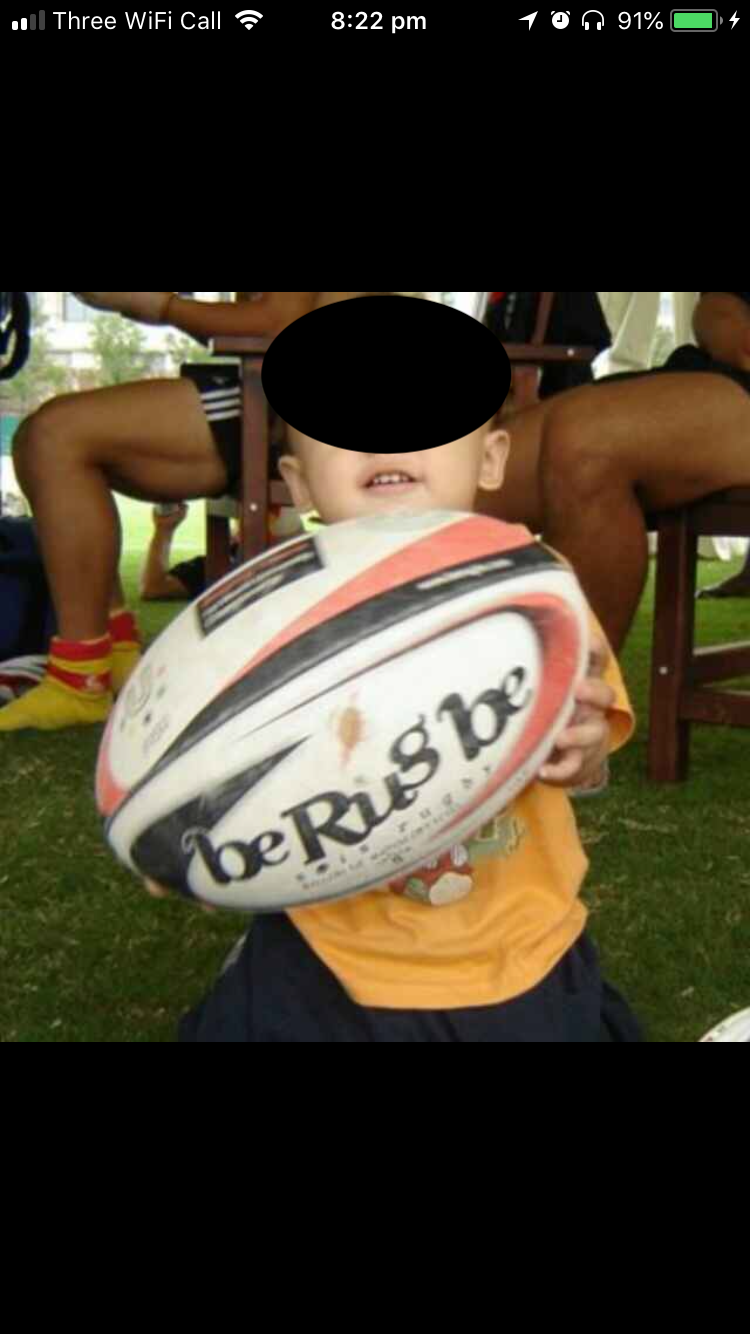
\includegraphics[scale =.2]{images/bjmWeChatProfile1.png}
      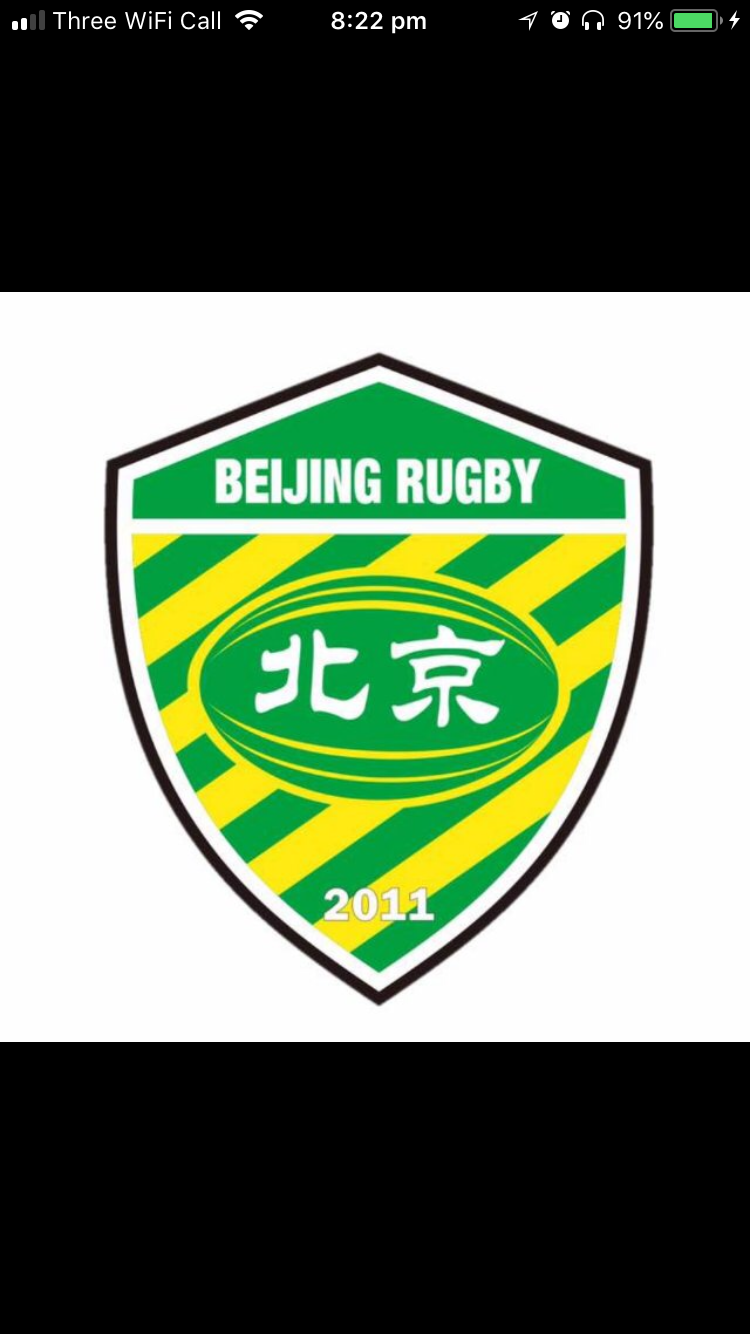
\includegraphics[scale =.2]{images/bjmWeChatProfile2.png}
      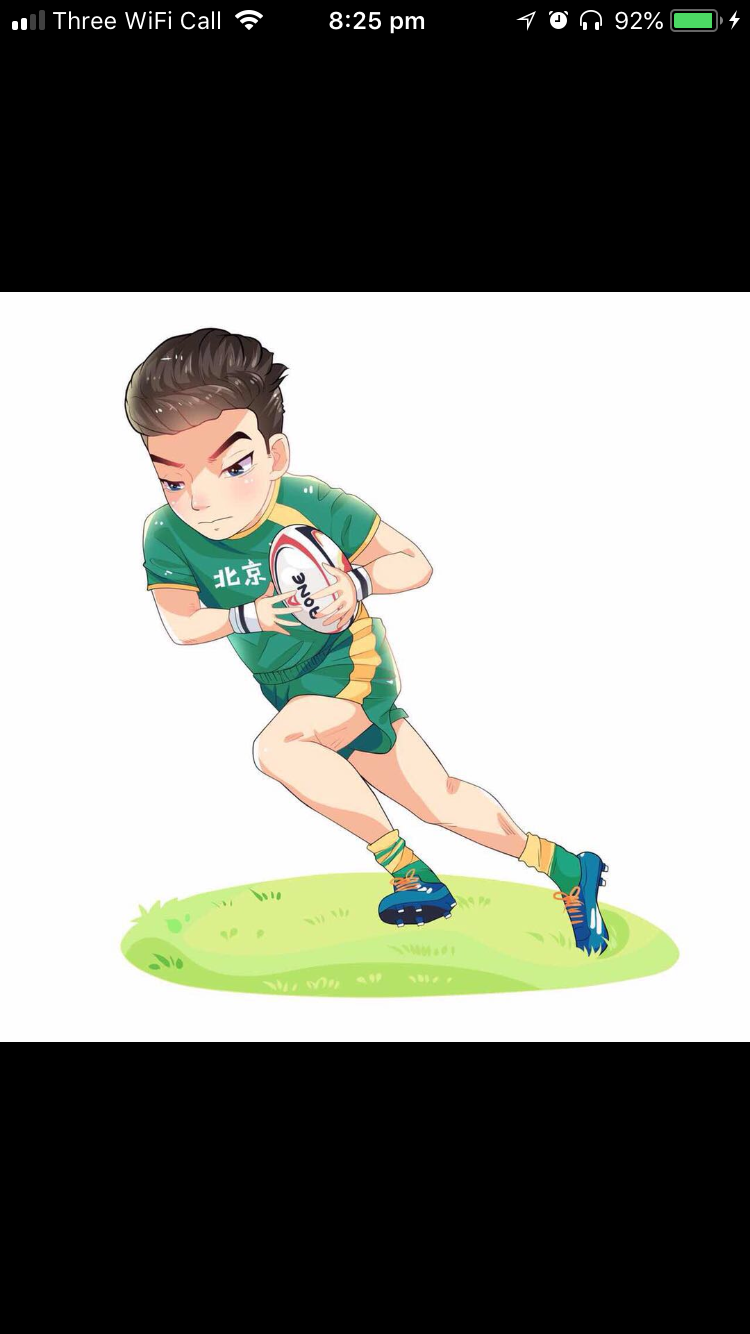
\includegraphics[scale =.2]{images/bjmWeChatProfile3.png}
      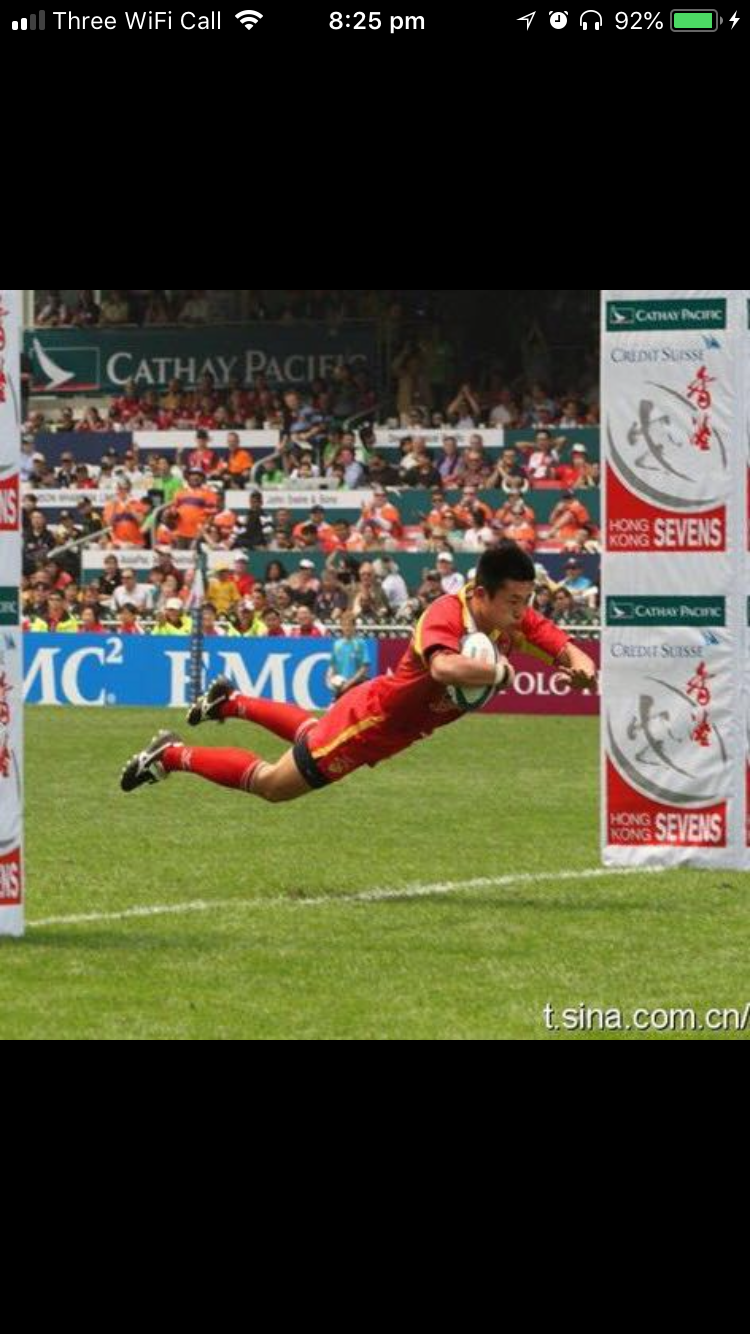
\includegraphics[scale =.2]{images/bjmWeChatProfile4.png}
      \caption{Screen shots taken from the social media profiles of a selection of athletes}
    \end{center}
      \label{fig:bjmWeChatProfile}
  \end{figure}

  %\myparagraph{Signalling on social media}
In addition to these explicit declarations recorded in interview settings, athletes' identification with the team and with rugby was evident from their use of other communication platforms.  Social media, for example, was a highly visible forum in which athletes would signal their social identity to friends and family.  Both junior and senior would display their connection to rugby on their individual WeChat accounts, by either changing their alias to include some reference to ``rugby'' or their profile picture, to display a photo of a rugby ball or a famous rugby player (see Figure ~\ref{fig:bjmWeChatProfile}).

Athletes commented to me that the rugby team at the Institute used to be the most formidable and successful team in the Institute, and that despite the recent fall from grace, the rugby team were still highly revered by the rest of the athletes at the Institute.  In the activity survey of motivations for adherence to rugby administered following semi-structured interviews (see Chapter ~\ref{chap:ethnoField} Section ~\ref{sect:athleteMotivation}), athletes on average cited ``to represent Beijing'' as their 4th highest ranked motivation for adherence to rugby, one spot below ``to gain respect.''  Both of these motivations show that adherence to rugby offers considerable social identity resources.

Ma Haitao explained to me the development of his feelings of belonging to the team:

  \begin{quote}
    When I first came my sense of belonging was not strong, in terms of joining the Beijing team, because I didn’t have anything, I couldn’t play! I wasn’t playing with the team, I wasn’t anything.  At the time in my heart I felt, being a Beijing Team member means going out and representing Beijing in a tournament.  If you haven’t represented Beijing then I felt like I hadn’t made a contribution, I could say to myself that I was part of the team, but I couldn’t actually recognise myself as being part of the Beijing team.  Now, last year when I played in a tournament, now I have that recognition. ``Are you in the Beijing team? Have you played in a tournament?'' (If the answer to these questions is) no, then I don’t recognise it myself.  Only last year after playing a Tournament did I slowly start recognising that I was part of Beijing team.
  \end{quote}

  \begin{quote}
    刚来的时候归属感不强,就加入北京队,因为什么都没有,啥都不会,没跟着一块打球,什么都不是。当时心里觉得什么是北京队,就是出去代表北京队比赛。没代表北京队就感觉自己也没为北京队做过贡献,说自己是北京队,自己都不认可自己是北京的。现在去年打比赛了,才对自己有认可。“你是北京队么?比过赛么?”没有。自己不认可。去年打完比赛才慢慢开始自己认可.
  \end{quote}

Ma explains that his ability to equate his personal identity with that of the Beijing team was contingent on him representing Beijing in national tournaments---before doing so he ``was nothing.''  This passage is a great demonstration of the power of the team as a coordinator and administrator of social identity.  It is interesting to note that for Ma, concrete on-field actions (taking the field for Beijing) signal authentic group membership.  Without the proven technical competence required to take the field for Beijing in a national tournament, Ma was unable to subscribe to Beijing rugby as a core personal identity.

%So what, then, of the situation involving the unacquainted fat kid who showed up a week before the final tournament in 2016?  Was he able to access the resources of social identity offered to him by virtue of him taking the field for Beijing? Or was his experience too momentary and ephemeral to allow for any lasting attachment?  I suggest his response to my questioning would have resembled one of the junior athletes, who tentatively suggests that rugby is fresh and enjoyable.

Senior athlete Wang Wei explains that his identification with rugby was a gradual process of familiarisation. Once familiarised, however, Wang came to like the sport in an irreversible sense:

  \begin{quote}
    I guess its exposure, when I first started my first impression was that it was barbaric, then after that slowly after more exposure to rugby I thought that this sport is really suited to males, I thought that this sport is a really good sport, I thought I had gradually come to like this sport.  At the beginning I thought it was too barbaric and wasn’t game to play, not game to tackle anyone to the ground or whatever, but after I’d been exposed to it for a long time, I came to understand the culture, and I came to like the sport.
  \end{quote}

  \begin{quote}
    还是接触吧,刚开始第一印象觉得野蛮,后来慢慢接触之后觉得这个项目挺适合男性运动,觉得这项目是个挺好的项目,觉得自己后来慢慢喜欢这个项目了。开始的时候觉得野蛮不敢打,不敢扑倒什么的,后来接触的时间长,了解这个文化了,就喜欢上这个东西了.
  \end{quote}

Wang recognises that identification with rugby requires time to develop. Through familiarisation with the technical and social affordances of rugby, athletes like Wang Wei and Haitao were able to gradually reconcile their personal identity with rugby.  Considered from an active inference paradigm, this progression from unfamiliar to familiar---embodied by the story of Sun Hongwei---could be evidence of the iterative strengthening of predictions at multiple levels of cognition, from the basal level of sensory routing and action plans in joint action, all the way up to the most abstract levels associated with group membership.



\myparagraph{Complete social and personal alignment with rugby}
Of all the athletes included in my analysis, senior athlete Han was perhaps the most explicit about the way in which rugby functioned as his social identity.  Han was the most experienced athlete and was also in a position in which he was uncertain about his future. What was certain, to Han at least, was that the only skills and resources he had to face the future were associated with rugby.   When I first arrived at the Institute, not knowing the details of the politics of the situation, I asked him what he was going to do next after the 2017 National Games.  Han smiled at me, recognising that at that time I had no idea about the details of his situation with the Leadership of the Institute. ``I don't know yet'' Han said to me, ``But all I know is that I just want to do this (rugby)'' (还没确定呢,我就想干这个).  Later in our semi-structured interview, Han explained his relationship to rugby in more detail:

    \begin{quote}
      HXL: I think its like this: as long as I like something, then I’m willing to commit to it.  And then I might get injured, or let myself get tired and fatigued or whatever, but I think ``I really like this sport, I am willing to do it.''\\
      JT: And once you come to like (rugby), these costs don't count as...\\
      HXL: Once you come to like rugby you're willing to invest a lot in it
    \end{quote}

    \begin{quote}
      HXL: 我觉得是这样,只要我喜欢这个东西,我就愿意去付出,然后可能会受伤啊、或者让自己很累很疲惫什么的,但是我觉得我挺喜欢这个项目,我愿意去做。\\
      JT: 喜欢了之后,这些成本不算...\\
      HXL: 喜欢之后可以付出很多.
    \end{quote}

Han's relationship to rugby represents another stage in the progression from complete novice to rugby master.  Xiaokai's explanations demonstrated a level of attachment to rugby, a feeling that it would be hard to leave, although leaving was still imaginable. Han's explanation, by contrast, showed a full realisation that his personal and social identity were aligned in a 1:1 ratio with rugby.

% as the theory of identity fusion would predict \cite{Swann2015}.

Senior athlete Lu Peng, the other remaining member of the old guard, also recognised that rugby represented his only viable path. Lu struck me as a viciously proud individual, and he was never as explicit as Han in his declarations of reliance on the team.  Instead, he would often emphasise his personal agency.  In our semi-structured interview, Lu explained to me his personal journey through the ranks of Chinese rugby, from CAU to the Institute:

\begin{quote}
    In those years at CAU (and you’d know this Li Jie), when I first arrived, I was not the focus of any nurturing, when I first arrived we were on the sidelines watching.  But I think [to myself] that I am different, my attitude is to think: ``I can, I can do it, I will be better than them.''\\

    When they [coaches and senior players] look at you and think ``oh ok you’ve just arrived,'' and maybe they say ``based on initial testing you’re good, you’re superior'' [motioning to other players]. But I think: I am good for it, I am better than them [those who had superior test results at the start].  But then based on a range of aspects the coach splits up the cohort into classes, and its those few athletes who tested well who will be nurtured, and we’re just average athletes.  It was very obvious. And then in my heart I was not satisfied, I thought I was stronger than them, and I wanted to dedicate myself to it.  And then I experienced a period of time when I expended a lot of effort, and I came a long way up.  Because at the start you are just an average person in their eyes, but then ultimately you get the opportunity through your own efforts. In my class (at Nongda) I should be (considered) the most outstanding.
\end{quote}

    \begin{quote}
    当年来农大我也挺励志的。在农大你应该知道,刚来的时候不是被重点培养的,刚来的在旁边看着,但是我觉我不一样,我的心态就是我觉得我可以,我能做到,我会比他们好...\\

    ...我就觉得,他们刚来的好,可能是他们确实刚来说测试你比较好,比较优秀,但是我觉得我可以,我比他们好。但是从各个方面他们教练就分出来等级的有他们比较好,是重点培养一些人,但是我们就是一般,很明显。然后我就很内心就是我不服,我觉得我比他们强,而且我要去做。然后经历了一段时间的努力付出然后超远上来了,因为刚开始你在他们眼里很一般的人,最终就是你通过自己的努力获得了机会。我现在就是我们班级,来一批,我应该最最优秀的。
    \end{quote}

On the face of it, Lu's disposition often appears to be rather anti-social---often critical of the others around him, and instead focussed on his own personal agency in the context of the team.  However Lu expressed it (i.e., whether via a focus on himself or talk of the team), during the many long discussions we had in my room, Lu would admit to me that rugby was his only viable future path.  After the 2017 national games he would attempt to keep playing for one more cycle, and then hopefully secure a job within the institute as a coach, or else look for a job elsewhere.  His family (wife and kids) were in Beijing, and he felt a certain amount of pressure to secure Beijing residency.  While Lu would not say so in the same way as Han, it was clear that rugby and the Beijing team meant a lot to him. Indeed, rugby defined who he was.  As mentioned above, it is inconceivable that someone not fused with the team would expend so much energy talking through ``every chicken feather and garlic peel'' (鸡毛蒜皮)---as Lu himself said it---of the Beijing rugby team with the resident anthropologist.

In these instances, athletes utilise both categories of the self and the team to describe the way in which participation in rugby has fostered an intensity of personal agency and group attachment.  (These two things are tethered and interdependent \citep{Kelso2016}).







\clearpage



\subsection{General Survey}

Results from an informal survey offer support for the observational and interview data reported above. I asked athletes to comment on experiences of joint action and group membership at two time points spread three months apart.  Athletes were asked to respond to questions about: experience of agency in the team (weak-strong), perceived role in the team (central-marginal), perceptions of individual performance (weak-strong), perceptions of team performance (weak-strong), training intensity (light-heavy) and difficulty (easy-hard).  All survey items were measured using a 7-point Likert scale.  The first general survey was administered at the end of November, approximately three months after I had begun fieldwork with the Beijing men's team.  I administered the same six questions at the beginning of February 2016, three months after the first survey and approximately one month after coach Wang had taken over as head coach of the team.

%(\textit{qiangdu} 强度)

%\begin{table}
  
% Please add the following required packages to your document preamble:
% \usepackage{booktabs}
\begin{table}[]
\centering
\begin{tabular}{@{}rclcl@{}}
\toprule
Survey Item                  & \multicolumn{2}{l}{November 2015} & \multicolumn{2}{l}{February 2016} \\ \midrule
\multicolumn{1}{c}{}         & Mean                    & SD      & Mean                    & SD      \\
\textbf{Training Intensity}  & \multicolumn{1}{l}{}    &         & \multicolumn{1}{l}{}    &         \\
Overall (n=23)               & \textbf{4.61}                   & 1.95    & \textbf{5.61}                    & 1.80    \\
Junior (n=13)                & \textbf{5.08}           & 2.18    & \textbf{6.23}           & 1.24    \\
Senior (n=10)                & \textbf{4.00}           & 1.49    & \textbf{4.80}           & 2.15    \\
\multicolumn{1}{l}{}         &                         &         &                         &         \\
\textbf{Training Difficulty} &                         &         &                         &         \\
Overall                      & 3.57                    & 1.44    & 3.70                    & 1.26    \\
Junior                       & 3.69                    & 1.84    & 3.54                    & 1.20    \\
Senior                       & 3.40                    & .70     & 3.90                    & 1.37    \\
\multicolumn{1}{l}{}         &                         &         & \multicolumn{1}{l}{}    &         \\
\textbf{Ind Perform}         &                         &         & \multicolumn{1}{l}{}    &         \\
Overall                      & 3.65                    & 1.30    & 3.57                    & 1.27    \\
Junior                       & 3.69                    & 1.38    & 3.60                    & 1.58    \\
Senior                       & 3.60                    & 1.2     & 3.54                    & 1.05    \\
\multicolumn{1}{l}{}         &                         &         & \multicolumn{1}{l}{}    &         \\
\textbf{Team Perform}        &                         &         & \multicolumn{1}{l}{}    &         \\
Overall                      & 3.83                    & 1.40    & 4.17                    & 1.44    \\
Junior                       & 4.00                    & 1.53    & 3.92                    & 1.26    \\
Senior                       & 3.60                    & 1.26    & 4.50                    & 1.65    \\
\multicolumn{1}{l}{}         &                         &         &                         &         \\
\textbf{Role in Team}        &                         &         &                         &         \\
Overall                      & 3.35                    & 1.43    & 3.35                    & 1.90    \\
Junior                       & \textbf{2.85}           & .90     & \textbf{2.92}           & 1.04    \\
Senior                       & \textbf{4.00}           & 1.76    & \textbf{3.90}           & 2.60    \\
\multicolumn{1}{l}{}         & \multicolumn{1}{l}{}    &         & \multicolumn{1}{l}{}    &         \\
\textbf{Agency}              & \multicolumn{1}{l}{}    &         & \multicolumn{1}{l}{}    &         \\
Overall                      & 3.26                    & 2.26    & 3.00                    & 2.17    \\
Junior                       & \textbf{2.31}           & 1.84    & \textbf{1.77}           & 1.25    \\
Senior                       & \textbf{4.50}           & 2.22    & \textbf{4.6}            & 2.12    \\ \bottomrule
\end{tabular}
\caption{Survey conducted at two times points, once in late November 2015 (during the leadership of Coach Zhu) and once in early Febrauary 2016 (during leadership of Coach Wang)}
\label{tab:groupMemBooktab}
\end{table}
%\end{table}


Table ~\ref{tab:groupMemBooktab} displays results of the surveys.  The only survey item that appears to vary according to time is the question concerning training intensity.  After Wang took over as coach he implemented a much more intense fitness regime.  Wang began to implement routine shuttle runs at the end of normal skills sessions, as well as weekly internal practice matches on Saturday morning (for example, the two training sessions after which I conducted the Flow State questionnaires).  These changes were perhaps partly motivated by a desire to differentiate his approach to training from his predecessor, but it was also due to the fact that after New Year the team entered the pre-season segment of training, whereas pre-Christmas training was well and truly classed as off-season. As Table ~\ref{tab:groupMemBooktab} indicates, the increase in perceptions of training intensity was driven by a larger increase in the junior athletes between the two time points.

The most striking results to emerge from the general surveys were the contrasts between junior and senior athlete reports of perceived position in the team and perceived agency in the team (the bottom two survey items in Table ~\ref{tab:groupMemBooktab}).  In both November 2016 and January 2017, junior athletes reported an average perceived agency of 2.31(1.84) and 1.77 (1.25) respectively. Senior athletes, by contrast, reported an average perceived agency of 4.50 (2.22) in November and 4.6 (2.12) in January.  Likewise, perceived position in the team showed similar differentials (see figures in bold in Table ~\ref{tab:groupMemBooktab}).  All other results, including perceptions of individual and team performance and training difficulty did not appear to vary by athlete group or by time.


\begin{figure}[htbp]
  \centering
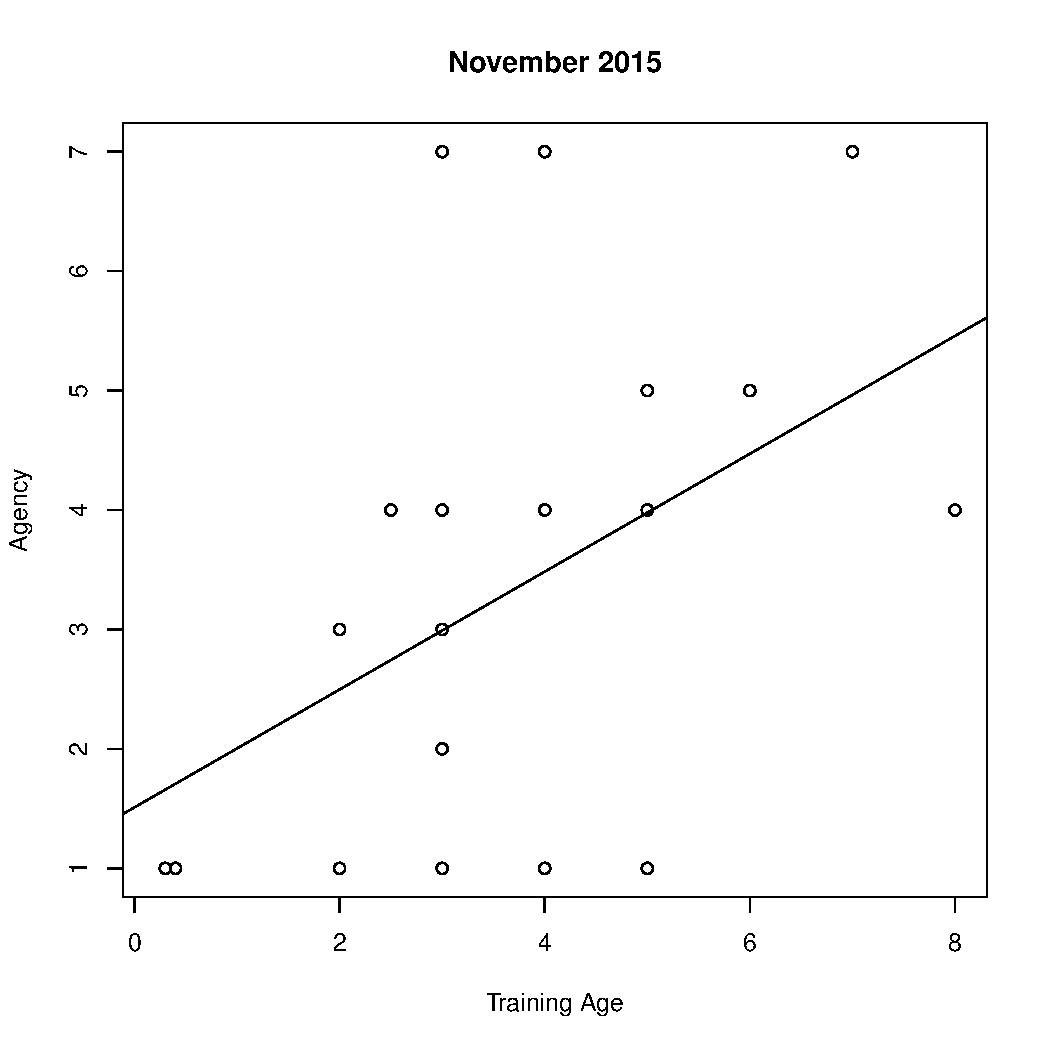
\includegraphics[scale=.3]{images/agencyTrainingNov.pdf}
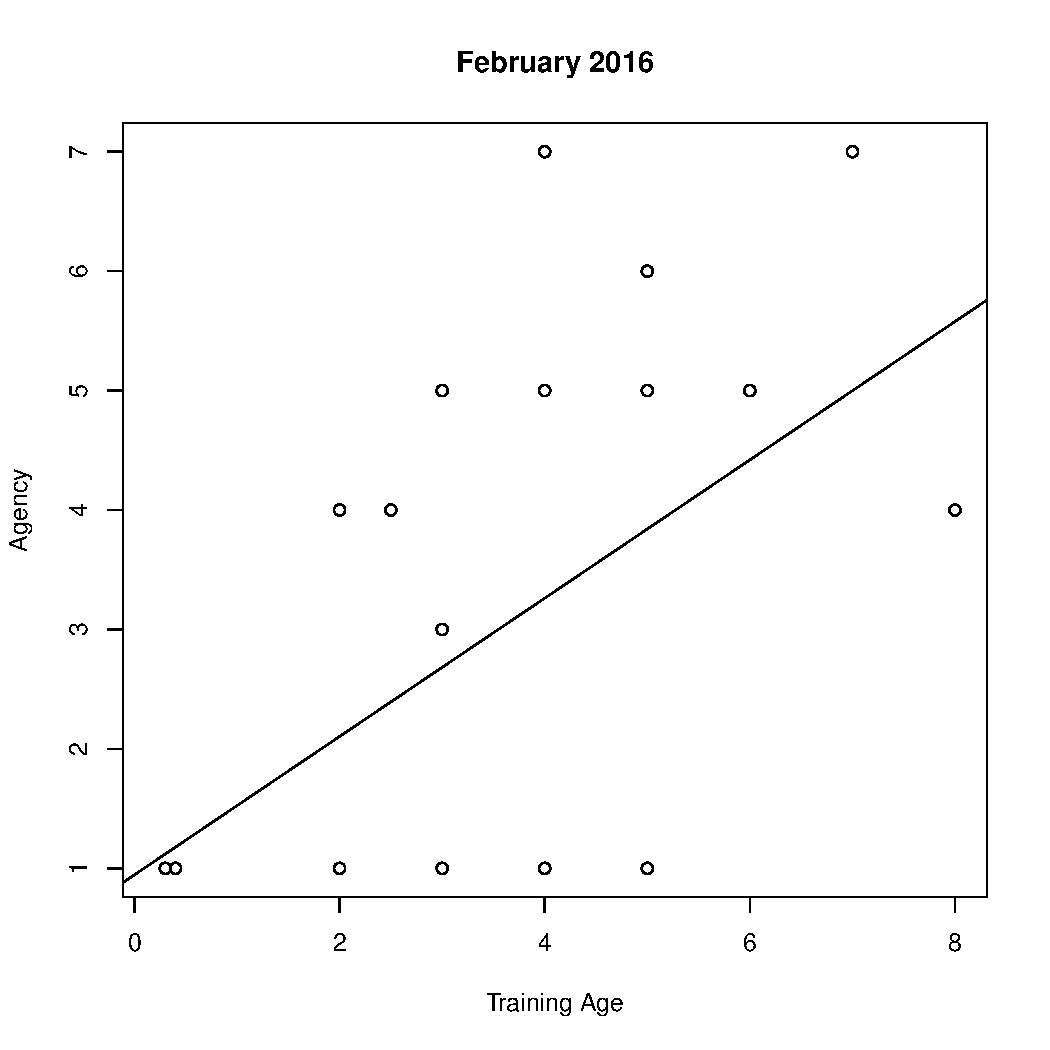
\includegraphics[scale=.3]{images/agencyTrainingFeb.pdf}
  \caption{Perceived agency in the team according to training age at two time points}
  \label{fig:agencyTrainingAge}
\end{figure}

\begin{figure}[htbp]
  \centering
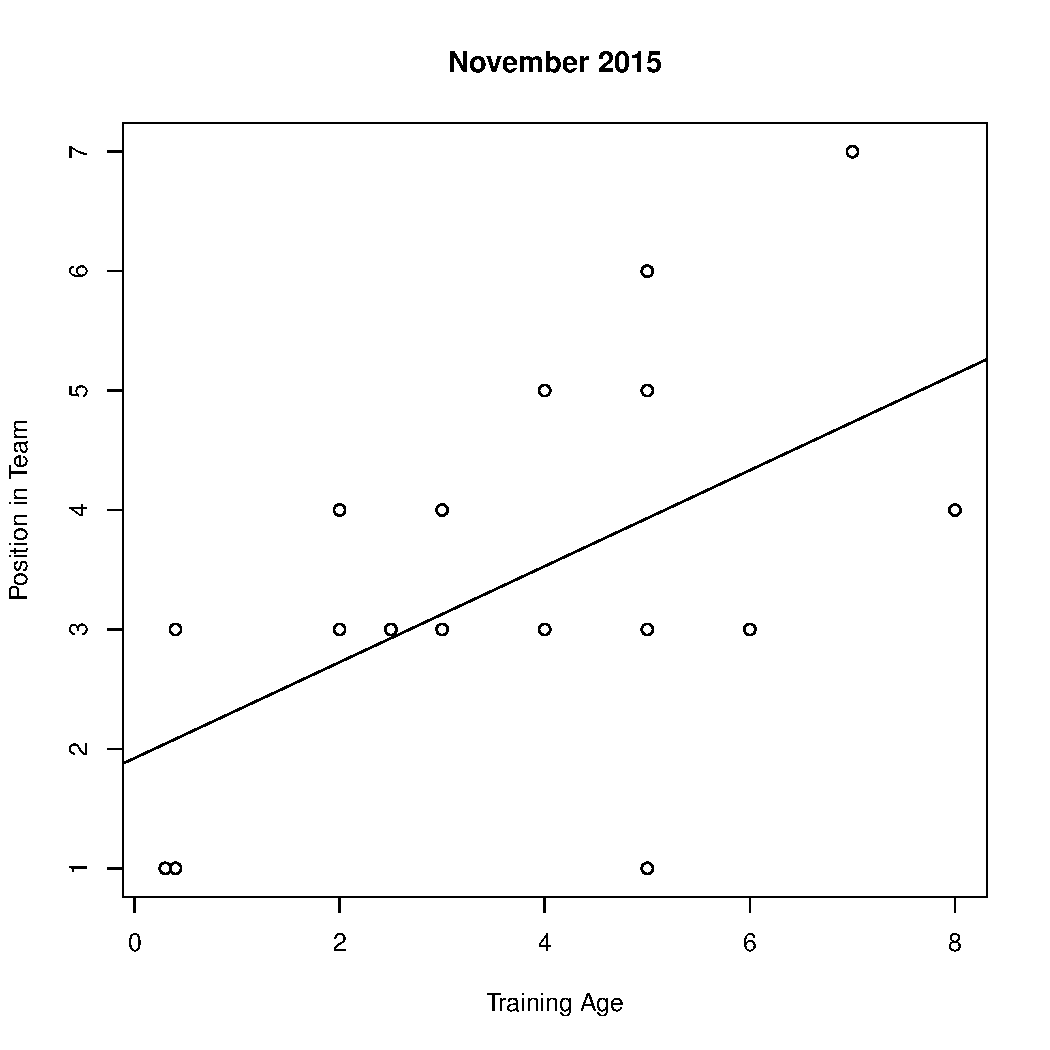
\includegraphics[scale=.3]{images/teamPosTrainingNov.pdf}
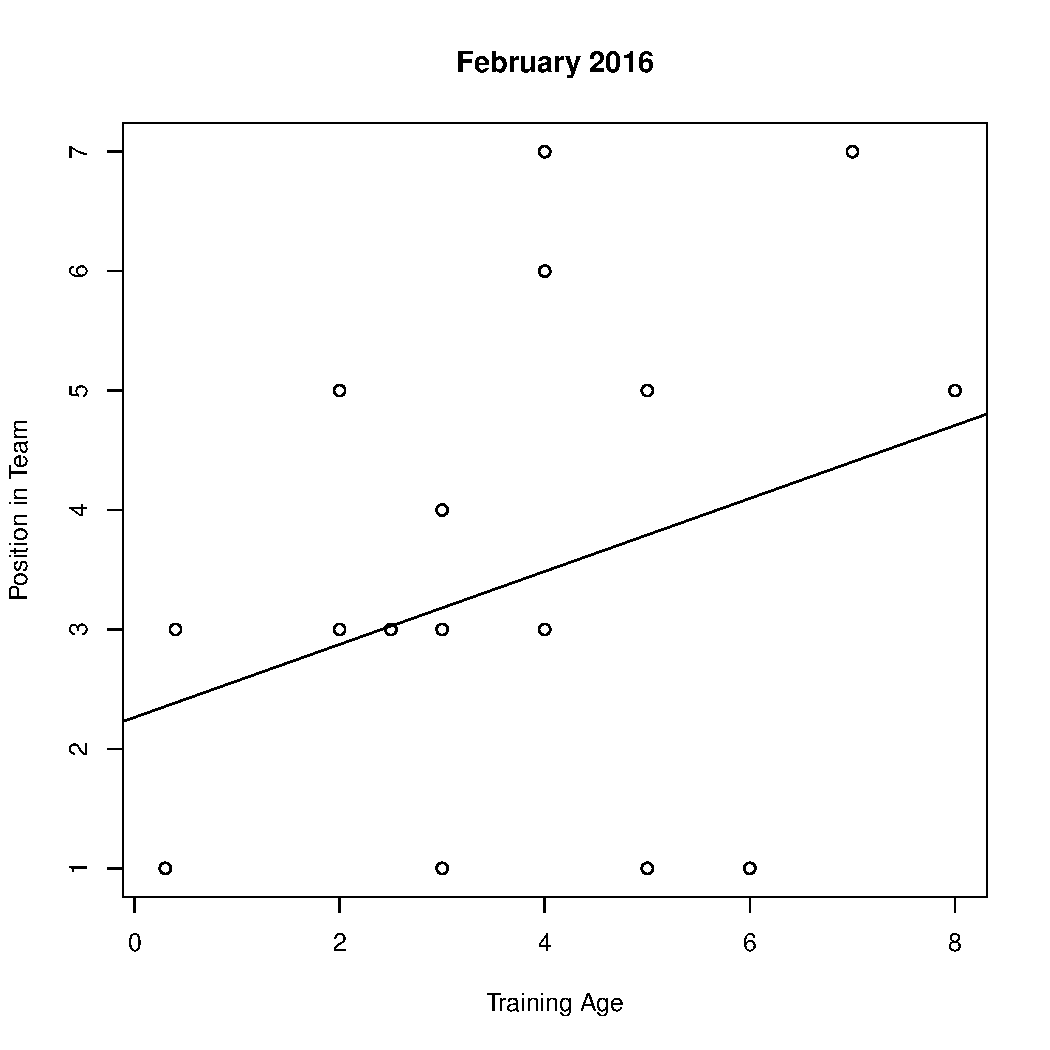
\includegraphics[scale=.3]{images/teamPosTrainingFeb.pdf}
  \caption{Perceived position team (central-peripheral) according to training age at two time points}
  \label{fig:teamPositionTrainingAge}
\end{figure}

Scatterplots reveal that perceptions of agency in the team and centrality of position in the team vary according to training age (see Figures ~\ref{fig:agencyTrainingAge} and ~\ref{fig:teamPositionTrainingAge}).

%Bring in semi-structured interview data about role in the team.



\clearpage




\subsection{Moderators\label{sect:mods}}

It is difficult through ethnographic observations alone to isolate the the various factors that influence processes of joint action and social bonding.  Ethnographic observations did provide evidence in line with predictions set out in Chapter ~\ref{chap:theory}, that entangled factors of age, experience, level of technical competence conditioned a relationship between joint action, team click, and social bonding.

        \subsubsection{Technical Competence}

In particular, more junior athletes appeared to be more emotional than senior athletes, when reflecting on performance, or reporting their experience of on field coordination or processes of group membership.


        \subsubsection{Personality\label{sect:ethnoPersonality}}

(Locus of control, focus on self versus others)
The team contained a range of personality types, from highly gregarious characters such as Lu Zhongsheng to more reserved characters like Yang Can.  Han versus Lu in the old guard.  In addition to age and status in the team, personality type could impact on the way in which athletes perceive performance and engage in group processes.

        \subsubsection{Injury}

Impact on confidence (Meng Cheng)
Ethnographic observations revealed that injury is a central feature of athlete experience, and can lead athletes to moderate their behaviour on the field and off the field.  Athletes reported the desire to mitigate the risk of injury by not committing to joint action with the same intensity that they may have usually (conservatism - Han Xiaolong).


        \subsubsection{Fatigue}

Athletes reported that physiological fatigue had an impact on their ability to maintain on-field awareness.  Fatigue could be an important moderator of joint action.

(When tired it affects vision and focus)
Fang Chao incident








\section{Discussion}

First statement:
  Layers of complexity in joint action in GE

Purpose of chapter:
  Ethnographic evidence of subjective experience of joint action.




Summarise results:
 I identify three core areas of analysis.  First, athletes pay close attention to their performance of joint action requirements specific to rugby union.  In particular, I notice that violation of athletes' expectations around joint action, both positive and negative, is a source of strong emotional response with implications for processes of group formation.  Second, ethnographic observations reveal that the experience of ``team click'' is a prominent experience in joint action associated with rugby, and appears to be connected in athletes' reasoning to concepts of team cohesion.  Third, I identify evidence of social bonding in processes of group formation.  In addition to these three core areas of ethnographic evidence, I also flag the possibility that these three processes are moderated by within-group variation in technical competence, personality type, injury, and athlete experience of fatigue and exertion in exercise.  I conclude this chapter by considering how these ethnographic data could be combined with existing theory and evidence and operationalised in further empirical studies beyond this specific ethnographic setting.

%Performance
  Athletes appear to develop strong subjective perceptions of individual and team performance, based on attention to specific technical components of rugby game play.   On the one hand, athletes display evidence of anxiety when expectations around individual and team performance are negatively violated.  When the same expectations concerning individual and team performance are positively violated, athletes are noticeably exhilarated, energised, and motivated.  Data collected in this ethnography suggest that more junior athletes appear more emotionally volatile when expressing perceptions of individual or team performance, such that both performance related anxiety and exhilaration appears to be more pronounced in junior athletes than senior athletes.  More senior athletes, by contrast, display the ability to relate to perceptions of individual and team performance expectations with more personal agency and emotional control.  More senior athletes talk in terms of an ability to strategically mitigate the costs of physical exertion and injury risk of joint action in rugby, whereas more junior athletes talk in less personal agency about their experience of individual and team performance.  These results suggest that perceptions of team and individual performance in joint action are formulated in relation to specific components of team and individual performance in joint action, as well as more general team and individual expectations structured by the specific team context, social norms, and institutional constraints.

%team click & bonding
  Athletes describe a number of phenomenological dimensions to optimal team performance (team click), including ``tacit understanding'' between teammates (\textit{moqi} 默契), ``team atmosphere,'' (\textit{qichang} 气场) and general order and structure to team coordination.  The data reveal within-group variation in the way athletes communicate team click: more junior athletes talk about team coordination in a more general and emotional way, whereas more senior athletes talk with a more restrained but more specific understanding of the dimensions and factors required in order to achieve peak team performance.  In regards to dimensions of social bonding, athletes appear to prioritise feelings of emotional support and a perception of a shared goal between teammates, as well as a level of personal connection to team roles and team identity.  Testimonies of team identity vary from the initial excitement and positivity of new arrivals towards, to the realisation of irreversible attachment to rugby of middle-rung athletes, to the out-and-out identity fusion between senior athletes and the practice of rugby, whereby athletes recognise that their self concept is inextricably linked with rugby and the Temple Institute.

%individual differences
  Finally, contained within the collected data is evidence that individual differences may moderate relationships between perceptions of joint action, team click, and social bonding.  Namely, an athlete's experience and competence with the technical and social dimensions of joint action of rugby at the Temple Institute may impact upon the ways in which they formulate and respond to expectations surrounding and team performance.  Individual differences in technical competence may also have flow-on effects for the formulation of feelings concerning team click and social bonding. It appears that individual personality types may moderate perceptions of performance in joint action, as well as feelings of team click and social bonding. In addition, other factors such as an athlete's injury status, and the level of fatigue and exertion experienced in joint action scenarios of rugby may impact on perceptions of performance, feelings of team click, and social bonding.  These individual differences should be considered in the design of quantitative studies to test the relationship between joint action, team click, and social bonding.



As explained above, social identity theory predicts that the individual derives social identity through a calculation of psychological distance between the category of self and the category of group.

The theory of hierarchical relationism, by contrast, starts from the default position that and social identity is realised through fostering a particularistic network of hierarchically structured relationships, and that categories of social identity are enlisted flexibly in service of these relationships.  As discussed in the previous chapter, within the particular setting of rugby in China, categories of self, other, and team appear to be porous.  At the level of the institution, the team, and even on-field joint action (see Chapter ~\ref{chap:ethnoField}), ethnographic evidence suggests the boundaries between these social categories are relaxed, to the extent that institutions (such as the institute or the Beijing rugby team) are not inherently stable or sanctimonious, and are rather platforms for social activity of particularistic networks of relationships.  Likewise, the category of the team is not inherently stable or sanctimonious, and motivation for team commitment relies on the alignment on various hierarchical levels of relationships, from the most junior athlete to the top of Leadership. On-field joint action, too, appears to be shaped by the priorities of preserving a relational order.

In a social setting in which hierarchical relationism is dominant, categories of self, other, and team are used flexibly in service of the more prominent goal of harmonising and fostering relationships, rather than relationships being used flexibly to reinforce categories of self and group.  In Han's captain's speech, for example, he utilised his personal identity as a vehicle to communicate an ultimately pro-social message (see Chapter ~\ref{chap:ethnoField} Section ~\ref{sect:IinTeam}).  His more junior athletes also demonstrated the prominence of the self in cultivating a public social identity, for example by emphasising the self-determination of their decision to play rugby (despite this decision also involving other agents such as their coach and their parents).  Indeed, it seemed that even Beijing's youngest rugby players lived in a world in which they were taught that the self (\textit{ziji} 自己) was the most important structure on which they had to rely see Chapter ~\ref{chap:ethnoField} Section ~\ref{sect:IinTeam}). More senior athletes show no reservation in crossing the boundaries of self and other in open scrutiny of athletes' on-field performance, and the chronic lack of communication in joint action also appears to demonstrate a lack of recognition that explicit messages need to travel between nodes in order for those nodes to communicate.  In fact, hierarchical relationism suggests a psychological state in which individuals already understand themselves to be fused with others in their immediate social environment---in which case explicit communication could be thought of as redundant.  In this sense, the Beijing rugby team is more resemblant of a nuclear family than it is an egalitarian forum for diverse independent interests. Regardless of its specific structure, provides athletes with resources to generate a social identity.




[AI]: reward for exploration and exploitation of new terrain Schwartenbeck2013


Identity requires reaching consensus between multiple hierarchical levels of self-concept: a multilevel click of layers of multimodal information (intero, proprio, extero).


Athletes appeared to flexibly utilise categories of self, team, and rugby more generally as a way of expressing their engagement with the sport.  Celebration of the category of the team featured strongly in interviews.  Given the personal nature of questioning, however, I also recorded many instances in which athletes described the way in which rugby featured as a space for self-validation and self understanding. The combination of ethnographic evidence I collected suggest that what varied within the group was not necessarily the psychological distance between the self and the group (as social identity theory would predict), but instead the level of (emotional) intensity of social identity derived from adherence to rugby, which could be flexibly expressed by calling upon either the category of self, the category of the team, or both.








                                                          \end{CJK}
